\chapter[Fundamentação Teórica]{Fundamentação Teórica}

Inicialmente, são discutidas a síntese de novas vistas, a reconstrução multivista a partir de imagens RGB e a distinção entre representações implícitas e explícitas. Em seguida, são apresentados os dois métodos centrais do pipeline, \textit{Neural Radiance Fields} (NeRF) e \textit{3D Gaussian Splatting} (3D-GS), bem como as restrições de Realidade Virtual autônoma, as métricas de avaliação, a plataforma Meta Quest 3S e as \textit{engines} consideradas para integração.

\section{Síntese de Novas Vistas e Representação de Cenas}

A síntese de novas vistas (\textit{Novel View Synthesis} -- NVS) busca gerar observações de uma cena a partir de poses de câmera não presentes no conjunto original. Esse problema dialoga com a renderização baseada em imagens, na qual a aparência da cena é descrita por amostras visuais e por sua variação com a posição e a direção de observação \cite{levoy1996lightfield,gortler1996lumigraph}. Em termos práticos, o objetivo é preservar geometria, aparência e consistência multivista ao produzir novas visualizações \cite{levoy1996lightfield,mildenhall2020,kerbl2023}.

Tradicionalmente, a NVS foi tratada por técnicas baseadas em geometria explícita, com uso de \textit{Structure-from-Motion} (SfM), \textit{Multi-View Stereo} (MVS), malhas e texturas. Apesar de consolidadas, essas abordagens podem ser instáveis em cenas com pouca textura, estruturas finas, reflexos, transparências ou forte dependência da iluminação, pois a qualidade final passa a depender das hipóteses de reconstrução e texturização \cite{seitz2006mvs,schoenberger2016sfm,mildenhall2020}.

Nesse contexto, a renderização neural ganhou relevância ao representar simultaneamente geometria aparente e radiância por funções aprendidas a partir de imagens calibradas \cite{sitzmann2019srn,mildenhall2020}. Entre essas abordagens, os \textit{Neural Radiance Fields} (NeRF) consolidaram a representação implícita de alta fidelidade, enquanto o \textit{3D Gaussian Splatting} (3D-GS) se destacou como alternativa explícita voltada à renderização em tempo real \cite{mildenhall2020,kerbl2023,fei2025survey3dgs}.

Neste trabalho, a síntese de novas vistas é analisada em relação a um objetivo aplicado: reconstruir cenas estáticas e torná-las visualizáveis em Realidade Virtual (VR) autônoma, cenário que exige qualidade visual, baixa latência e renderização interativa \cite{xu2023,tu2025,metaquest3s2024}.

\section{Reconstrução Multivista a partir de Imagens RGB}

A reconstrução de cenas a partir de imagens RGB parte do princípio de que diferentes observações bidimensionais de uma mesma cena contêm redundância geométrica e fotométrica suficiente para inferir sua estrutura tridimensional. Para isso, as imagens devem apresentar cobertura espacial, sobreposição entre vistas e diversidade de poses de câmera, reduzindo ambiguidades geométricas e preservando paralaxe \cite{seitz2006mvs,schoenberger2016sfm}.

Nos fluxos modernos de reconstrução neural, a preparação dos dados permanece essencial. Mesmo quando a cena final é representada por um campo neural ou por gaussianas explícitas, a consistência entre imagens depende das poses e dos parâmetros intrínsecos de câmera, normalmente estimados por pipelines de calibração e reconstrução multivista \cite{schoenberger2016sfm,mildenhall2020,kerbl2023}.

A Figura \ref{fig:reconstrucao_multivista_pipeline} sintetiza esse fluxo de reconstrução multivista, evidenciando a relação entre correspondência entre imagens, registro incremental das câmeras e recuperação da estrutura da cena, etapas associadas ao processo de SfM incremental descrito por \citeonline{schoenberger2016sfm}.

\begin{figure}[H]
    \centering
    \fbox{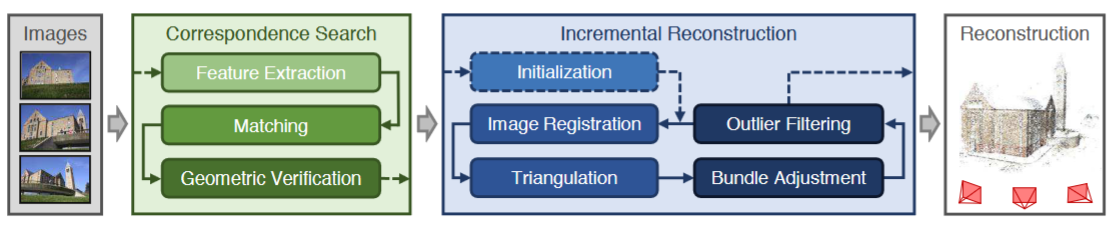
\includegraphics[width=\textwidth]{figuras/incremental_sfm_pipeline.png}}
    \caption{Etapas conceituais da reconstrução multivista, desde a correspondência entre imagens até a recuperação da estrutura da cena e das poses de câmera.}
    \label{fig:reconstrucao_multivista_pipeline}
    \fonte{Adaptado de \cite{schoenberger2016sfm}.}
\end{figure}

Conceitualmente, essa etapa conecta o domínio das imagens ao domínio da cena: as fotografias precisam ser interpretadas como amostras coerentes de uma mesma estrutura espacial. Essa premissa delimita o escopo deste trabalho a cenas estáticas capturadas por imagens RGB, excluindo dinâmicas 4D, \textit{relighting} complexo e outros fatores que ampliariam a ambiguidade do problema \cite{seitz2006mvs,schoenberger2016sfm,xu2023}.

Em cenas estáticas, a consistência entre observações permite agregar diferentes imagens no aprendizado de uma representação única. Assim, a preparação dos dados não é apenas operacional, mas condição para comparar representações implícitas e explícitas no pipeline proposto \cite{sitzmann2019srn,mildenhall2020,kerbl2023,fei2025survey3dgs}.

\subsection{Representações implícitas}

Representações implícitas descrevem uma cena por funções contínuas definidas sobre o espaço, em vez de armazená-la diretamente como uma coleção de vértices, superfícies ou primitivas geométricas. Nesse paradigma, a cena é codificada nos parâmetros de uma função aprendida, capaz de receber coordenadas espaciais e retornar propriedades locais, como densidade, ocupação, cor ou radiância \cite{sitzmann2019srn,mildenhall2020}.

A continuidade dessas representações permite consultar a cena em posições arbitrárias, favorecendo interpolação suave, modelagem de detalhes e consistência multivista. Também permite representar estruturas complexas sem depender de malhas bem definidas ou topologias rígidas, característica explorada por redes de representação de cena e consolidada pelo NeRF \cite{sitzmann2019srn,mildenhall2020,barron2021mipnerf}.

Como limitação, a cena não está materializada em uma estrutura discreta, e a renderização depende de consultas repetidas à função aprendida. No NeRF, por exemplo, cada pixel exige integração volumétrica ao longo de um raio, com múltiplas amostragens e inferências sucessivas \cite{mildenhall2020,muller2022}. Mesmo com acelerações, esse custo dificulta a renderização interativa em hardware restrito \cite{muller2022,xu2023}, o que motiva a análise de representações explícitas \cite{kerbl2023,fei2025survey3dgs}.

\subsection{Representações explícitas}

Representações explícitas armazenam a cena em estruturas discretas diretamente manipuláveis pelo pipeline gráfico, como malhas, nuvens de pontos, voxels e primitivas volumétricas projetáveis. Por associarem geometria e aparência a entidades concretas, tendem a facilitar integração com motores gráficos, rasterização e visualização em tempo real \cite{zwicker2001,kerbl2023,fei2025survey3dgs}.

A principal vantagem desse paradigma está na eficiência de renderização, pois os elementos da cena já se encontram organizados em estruturas compatíveis com técnicas gráficas tradicionais. O \textit{3D Gaussian Splatting} insere-se nesse contexto ao representar a cena por gaussianas anisotrópicas projetadas e compostas no plano da imagem \cite{kerbl2023}, favorecendo aplicações interativas \cite{kerbl2023,fei2025survey3dgs}.

Por outro lado, representações explícitas exigem maior cuidado com organização estrutural, gerenciamento de memória e adequação da quantidade de primitivas à complexidade da cena. Em cenários extensos ou detalhados, o número de elementos pode crescer substancialmente, elevando consumo de armazenamento, largura de banda e memória de vídeo \cite{fei2025survey3dgs,wu2025,fang2024,huang2025}.

Assim, o custo principal desloca-se das consultas de inferência para armazenamento, organização e seleção de primitivas \cite{mildenhall2020,kerbl2023,fei2025survey3dgs}.

\subsection{Comparação entre os paradigmas}

A comparação entre representações implícitas e explícitas envolve um \textit{trade-off} entre continuidade funcional e eficiência estrutural. Representações implícitas favorecem modelagem contínua e síntese visual de alta qualidade, mas costumam apresentar custo de inferência elevado \cite{sitzmann2019srn,mildenhall2020,muller2022}.

Representações explícitas favorecem velocidade de renderização e integração com pipelines gráficos convencionais, mas demandam estratégias de escalabilidade, poda, compressão e seleção de nível de detalhe quando executadas em plataformas restritas \cite{kerbl2023,fei2025survey3dgs,wu2025,fan2024lightgaussian}.

Outra diferença está no acesso à geometria. Em representações implícitas, ela emerge indiretamente da função aprendida; nas explícitas, os elementos da cena são acessíveis como primitivas discretas, facilitando manipulação, inspeção e integração com sistemas gráficos \cite{sitzmann2019srn,mildenhall2020,kerbl2023,fei2025survey3dgs}.

\subsection{Relação com o escopo deste trabalho}

No contexto deste trabalho, essa distinção estrutura o pipeline proposto. O NeRF é adotado como referência de reconstrução de cenas estáticas, enquanto o 3D Gaussian Splatting é investigado como representação explícita mais compatível com renderização interativa em Realidade Virtual \cite{sitzmann2019srn,mildenhall2020,kerbl2023,xu2023,tu2025}.

Dessa forma, o problema investigado consiste em articular dois paradigmas no mesmo fluxo de reconstrução e visualização, equilibrando qualidade visual e desempenho em hardware VR autônomo \cite{muller2022,kerbl2023,xu2023,metaquest3s2024}.

\section{Neural Radiance Fields}

No contexto das representações implícitas, os \textit{Neural Radiance Fields} (NeRF) constituem um marco da síntese de novas vistas por modelarem cenas complexas como funções contínuas aprendidas. Essa abordagem se insere em uma trajetória de representações neurais de cena que inclui SRNs e variantes posteriores voltadas a eficiência e antialiasing multiescala \cite{sitzmann2019srn,mildenhall2020,barron2021mipnerf}. Neste trabalho, o NeRF é adotado como referência conceitual e técnica para a etapa de reconstrução.

\subsection{Representação implícita da cena}

Os \textit{Neural Radiance Fields} modelam uma cena como uma função contínua de radiância e densidade. Em sua formulação clássica, um MLP recebe como entrada uma posição espacial $\mathbf{x} = (x,y,z)$ e uma direção de visualização $\mathbf{d}$, retornando uma densidade volumétrica $\sigma$ e uma cor $\mathbf{c}$ dependente da vista \cite{sitzmann2019srn,mildenhall2020}. Formalmente, essa relação pode ser expressa por:

\begin{equation}
F_{\Theta}(\mathbf{x}, \mathbf{d}) \rightarrow (\sigma, \mathbf{c})
\label{eq:nerf_funcao}
\end{equation}
\addEquacao{Mapeamento da função \textit{radiance field}}{\ref{eq:nerf_funcao}}

em que $\Theta$ representa os parâmetros aprendidos da rede. A densidade $\sigma$ atua como uma medida da probabilidade de ocupação local ao longo do espaço, enquanto a cor representa a radiância emitida na direção de observação. Essa formulação é chamada de implícita porque a geometria da cena não é armazenada explicitamente como uma malha, nuvem de pontos ou conjunto de primitivas, mas sim codificada nos parâmetros da função aprendida \cite{sitzmann2019srn,mildenhall2020}.

Essa formulação permite consultar a cena em coordenadas arbitrárias, favorecendo suavidade espacial e coerência geométrica. Ao mesmo tempo, dificulta o acesso direto à estrutura da cena e impõe custo de inferência, pois a imagem depende de múltiplas consultas à rede para cada raio de câmera \cite{mildenhall2020,muller2022}.

\subsection{Renderização volumétrica}

A imagem final em NeRF é obtida por renderização volumétrica. Para cada pixel, considera-se um raio que parte da câmera e atravessa a cena, sendo parametrizado por uma origem $\mathbf{o}$, uma direção $\mathbf{d}$ e uma distância escalar $t$ ao longo do raio \cite{mildenhall2020,barron2021mipnerf}. Essa parametrização é dada por:

\begin{equation}
\mathbf{r}(t) = \mathbf{o} + t\mathbf{d},
\label{eq:raio_parametrizado}
\end{equation}
\addEquacao{Parametrização do raio}{\ref{eq:raio_parametrizado}}

A cor esperada de um raio é calculada pela integração da radiância e da densidade volumétrica ao longo do intervalo entre os limites próximo e distante da cena. Nessa formulação, a contribuição de cada ponto depende tanto da cor emitida naquela posição quanto da probabilidade de o raio alcançá-la sem ter sido absorvido anteriormente \cite{mildenhall2020,barron2021mipnerf}. Formalmente, essa cor é dada por:

\begin{equation}
C(\mathbf{r}) = \int_{t_n}^{t_f} T(t)\sigma(\mathbf{r}(t))\mathbf{c}(\mathbf{r}(t),\mathbf{d})\,dt,
\label{eq:cor_raio_integral}
\end{equation}
\addEquacao{Cor esperada de um raio por renderização volumétrica}{\ref{eq:cor_raio_integral}}

Na Equação \ref{eq:cor_raio_integral}, o termo $T(t)$ corresponde à transmitância acumulada ao longo do raio, isto é, à probabilidade de que o raio percorra o caminho entre o limite inicial $t_n$ e a posição $t$ sem ser interrompido por densidade volumétrica relevante \cite{mildenhall2020,barron2021mipnerf}. Esse termo é definido por:

\begin{equation}
T(t) = \exp\left(-\int_{t_n}^{t}\sigma(\mathbf{r}(s))\,ds\right).
\label{eq:transmitancia}
\end{equation}
\addEquacao{Transmitância acumulada ao longo do raio}{\ref{eq:transmitancia}}

Na prática, a integral contínua da renderização volumétrica é aproximada numericamente por meio de amostras discretas ao longo do raio. Esse processo transforma a integral em uma soma ponderada das cores estimadas em diferentes pontos, considerando a opacidade e a transmitância acumulada em cada amostra \cite{mildenhall2020,barron2021mipnerf}. Uma forma comum dessa discretização é:

\begin{equation}
\hat{C}(\mathbf{r}) = \sum_{i=1}^{N} T_i \alpha_i \mathbf{c}_i,
\label{eq:cor_discreta}
\end{equation}
\addEquacao{Aproximação discreta da cor do raio}{\ref{eq:cor_discreta}}

A opacidade associada a cada amostra é calculada a partir da densidade volumétrica estimada pela rede e da distância entre amostras consecutivas. Esse procedimento aproxima o processo de composição alfa utilizado na renderização volumétrica clássica, permitindo que a formulação seja diferenciável e, portanto, adequada ao treinamento por otimização baseada em erro fotométrico \cite{mildenhall2020,barron2021mipnerf}. A opacidade de cada amostra é dada por:

\begin{equation}
\alpha_i = 1 - \exp(-\sigma_i \delta_i),
\label{eq:opacidade_amostra}
\end{equation}
\addEquacao{Opacidade associada a cada amostra}{\ref{eq:opacidade_amostra}}

em que $\delta_i$ representa a distância entre amostras consecutivas. Essa formulação explica o principal custo computacional do NeRF: para cada pixel é necessário consultar vários pontos no espaço e acumular os resultados. Em alta resolução ou renderização estereoscópica, o número de raios e amostras cresce rapidamente \cite{mildenhall2020,xu2023}.

\subsection{Codificação posicional e amostragem hierárquica}

O NeRF clássico introduziu dois mecanismos importantes para melhorar a reconstrução: codificação posicional e amostragem hierárquica. A codificação posicional projeta coordenadas de baixa dimensão em um espaço de frequências mais altas, permitindo ao MLP representar detalhes finos de textura e geometria, em consonância com a análise de \citeonline{tancik2020fourier} sobre características de Fourier \cite{mildenhall2020,tancik2020fourier}.

A amostragem hierárquica distribui melhor o esforço computacional ao concentrar amostras adicionais nas regiões do raio com maior contribuição para a imagem. Embora reduza parte da ineficiência, o custo de inferência permanece relevante quando comparado a métodos baseados em rasterização explícita \cite{mildenhall2020,kerbl2023}.

\subsection{Avanços práticos e limitações}

Após a formulação original, surgiram variantes voltadas à aceleração do treinamento e da inferência. Entre elas, destaca-se o Instant-NGP, que substitui a dependência exclusiva de um MLP profundo por uma codificação hash multirresolução, reduzindo expressivamente o tempo de treinamento sem abandonar a formulação de campo neural \cite{muller2022}.

Mesmo com acelerações relevantes, o paradigma volumétrico continua mais custoso do que representações explícitas quando o objetivo é renderização interativa em alta frequência. Assim, o NeRF permanece valioso como linha de base de fidelidade visual, mas encontra limitações sob restrições de memória, consumo e latência \cite{muller2022,yu2021plenoctrees,hedman2021snerg,kerbl2023}.

Essa limitação justifica a análise de alternativas explícitas, como o \textit{3D Gaussian Splatting}, capazes de aproximar a síntese de vistas de um regime mais compatível com renderização interativa \cite{yu2021plenoctrees,hedman2021snerg,kerbl2023,fei2025survey3dgs}.

\section{3D Gaussian Splatting}

Em contraste com o NeRF, o \textit{3D Gaussian Splatting} (3D-GS) representa a cena por primitivas explícitas diretamente manipuláveis no espaço tridimensional. Sua relevância está em combinar qualidade visual com renderização eficiente, característica central para aplicações interativas e para o escopo deste trabalho \cite{mildenhall2020,muller2022,kerbl2023,fei2025survey3dgs,chen2024survey3dgs}.

Sua emergência acompanha uma trajetória de aceleração da síntese de vistas, da qual também fazem parte Instant-NGP, PlenOctrees e SNeRG \cite{mildenhall2020,muller2022,yu2021plenoctrees,hedman2021snerg}. O diferencial do 3D-GS está em deslocar a unidade elementar da cena para gaussianas explícitas, mantendo otimização diferenciável e renderização por rasterização \cite{kerbl2023,fei2025survey3dgs,chen2024survey3dgs}. 

A Figura \ref{fig:3dgs_qualidade_velocidade} sintetiza essa comparação ao relacionar qualidade visual, tempo de treinamento e taxa de renderização, destacando o 3D-GS como uma alternativa situada no compromisso entre alta fidelidade e execução interativa \cite{kerbl2023}.

\begin{figure}[H]
    \centering
    \fbox{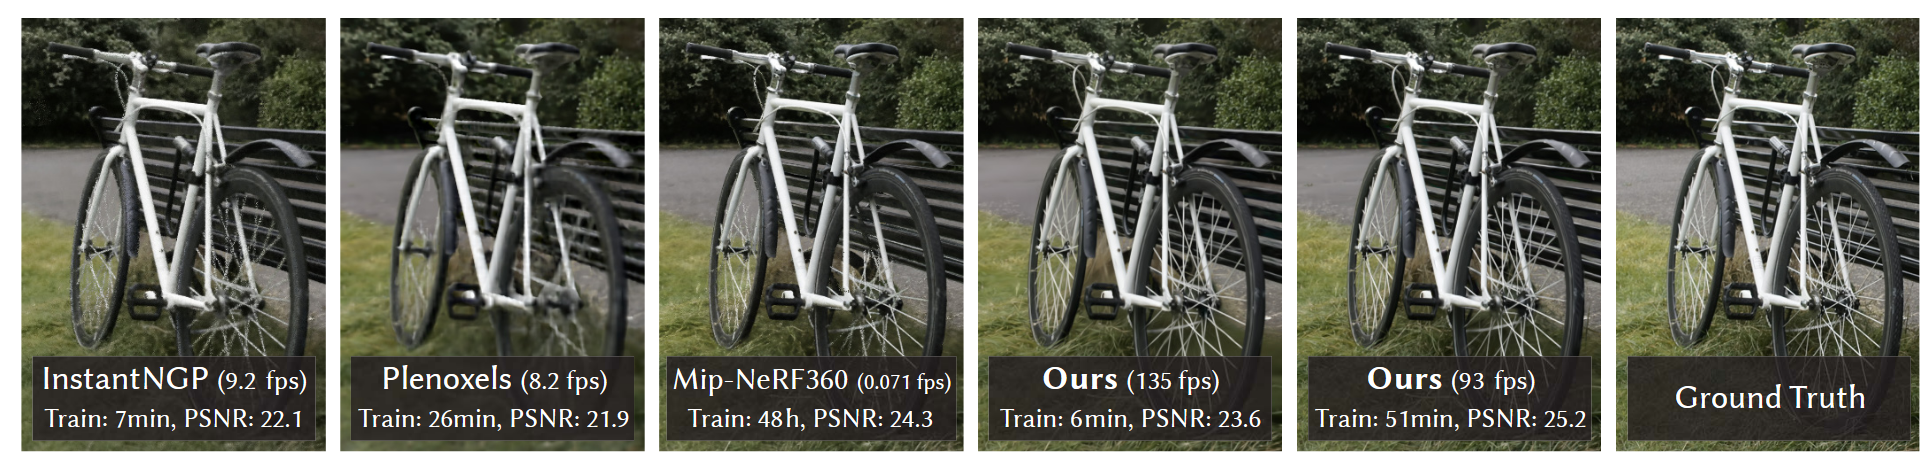
\includegraphics[width=\textwidth]{figuras/kerbl2023_fig1.png}}
    \caption{Comparação ilustrativa entre métodos de síntese de novas vistas, evidenciando o compromisso entre qualidade visual, tempo de treinamento e taxa de renderização.}
    \label{fig:3dgs_qualidade_velocidade}
    \fonte{Adaptado de \cite{kerbl2023}.}
\end{figure}

\subsection{Representação explícita por gaussianas anisotrópicas}

O \textit{3D Gaussian Splatting} descreve a cena por gaussianas anisotrópicas parametrizadas por posição, escala, rotação, opacidade e aparência dependente da vista \cite{kerbl2023,fei2025survey3dgs,chen2024survey3dgs}. Assim, a cena pode ser otimizada a partir de imagens calibradas e renderizada por um processo mais próximo dos pipelines gráficos tradicionais.

Cada gaussiana é uma distribuição espacial contínua centrada em $\boldsymbol{\mu}$, cuja forma é controlada por uma matriz de covariância $\Sigma$. Essa estrutura representa regiões locais como elipsoides orientados, adaptáveis a superfícies inclinadas, estruturas alongadas e detalhes geométricos finos \cite{kerbl2023,zwicker2001,chen2024survey3dgs}. Formalmente, uma gaussiana tridimensional pode ser escrita como:

\begin{equation}
G(\mathbf{x}) =
\exp\left(
-\frac{1}{2}
(\mathbf{x} - \boldsymbol{\mu})^{T}
\Sigma^{-1}
(\mathbf{x} - \boldsymbol{\mu})
\right).
\label{eq:gaussiana_3d}
\end{equation}
\addEquacao{Distribuição espacial de uma gaussiana anisotrópica}{\ref{eq:gaussiana_3d}}

Para garantir estabilidade numérica e positividade da covariância, a matriz $\Sigma$ é fatorada em termos de rotação e escala. Essa parametrização evita otimizar diretamente uma matriz de covariância arbitrária e preserva a interpretação geométrica da primitiva \cite{kerbl2023,chen2024survey3dgs}. A fatoração pode ser expressa por:

\begin{equation}
\Sigma = R S S^{T} R^{T},
\label{eq:fatoracao_covariancia}
\end{equation}
\addEquacao{Fatoração da matriz de covariância em rotação e escala}{\ref{eq:fatoracao_covariancia}}

em que $R$ representa a rotação e $S$ codifica a escala da primitiva. Além da geometria local, cada gaussiana armazena opacidade e parâmetros de aparência. A aparência dependente da vista é usualmente modelada por harmônicos esféricos, aproximando variações angulares de cor sem reintroduzir uma rede neural volumétrica custosa na renderização \cite{kerbl2023,yu2021plenoctrees,fei2025survey3dgs}.

Conceitualmente, o 3D-GS pode ser visto como uma nuvem de pontos enriquecida, na qual cada ponto se torna uma primitiva volumétrica suave, orientada e otimizável. Isso permite preencher lacunas visuais e reduzir descontinuidades, retomando princípios de \textit{splatting} elíptico em renderização baseada em pontos \cite{zwicker2001,kerbl2023,chen2024survey3dgs}.

\subsection{Splatting, projeção e composição de cor}

A formação de imagem no 3D-GS ocorre por projeção das gaussianas 3D no plano da imagem e composição por transparência. Esse princípio dialoga com trabalhos clássicos de \textit{splatting} e filtragem elíptica \cite{zwicker2001}, mas é incorporado a um pipeline diferenciável otimizado para síntese de novas vistas a partir de imagens calibradas \cite{kerbl2023,fei2025survey3dgs}.

A projeção transforma cada gaussiana em uma contribuição elíptica no plano da imagem. Em termos gerais, a covariância tridimensional é levada ao espaço da câmera e aproximada no plano de projeção, de modo que cada primitiva contribua apenas para os pixels cobertos \cite{kerbl2023,chen2024survey3dgs}. 

Enquanto o NeRF calcula cada pixel por amostragem ao longo de raios lançados pela câmera, o 3D-GS projeta diretamente suas gaussianas 3D no plano da imagem, rasterizando suas contribuições elípticas sobre os pixels cobertos, uma estratégia chamada de \textit{forward mapping} \cite{mildenhall2020,kerbl2023,chen2024survey3dgs}.

Após a projeção para o espaço 2D, as gaussianas visíveis são ordenadas por profundidade e compostas no pixel por um processo análogo ao \textit{alpha blending}. Em formulação simplificada, a cor final pode ser descrita por:

\begin{equation}
C = \sum_{i \in \mathcal{N}} c_i \alpha_i \prod_{j=1}^{i-1}(1-\alpha_j),
\label{eq:composicao_cor_3dgs}
\end{equation}
\addEquacao{Composição de cor por transparência no 3D-GS}{\ref{eq:composicao_cor_3dgs}}

em que $c_i$ é a contribuição cromática da $i$-ésima gaussiana e $\alpha_i$ sua opacidade efetiva sobre o pixel. Essa formulação é próxima à composição volumétrica utilizada em NeRF, mas com uma diferença estrutural importante: o 3D-GS modela diretamente opacidade e aparência nas primitivas projetadas, enquanto o NeRF converte densidade em opacidade por meio de amostras ao longo dos raios \cite{mildenhall2020,kerbl2023,fei2025survey3dgs}.

Diferentemente do NeRF, o 3D-GS não exige amostrar densamente o espaço ao longo de cada raio. A renderização se apoia em rasterização diferenciável, organização por \textit{tiles}, ordenação por profundidade e composição paralela, tornando o método mais compatível com GPUs modernas \cite{kerbl2023,chen2024survey3dgs}.

\subsection{Otimização, densificação e poda}

Um aspecto central do 3D-GS é o uso de densificação e poda durante o treinamento. Diferentemente de uma malha fixa ou de uma nuvem de pontos estática, o conjunto de gaussianas evolui: primitivas podem ser divididas, ajustadas ou removidas conforme sua contribuição para a síntese \cite{kerbl2023,fei2025survey3dgs,chen2024survey3dgs}.

No trabalho original, a otimização combina uma perda fotométrica em norma $L_1$ com um termo baseado em D-SSIM, equilibrando fidelidade por pixel e preservação estrutural da imagem \cite{kerbl2023,wang2004}. De forma simplificada, a função de perda pode ser expressa como:

\begin{equation}
\mathcal{L}
=
(1-\lambda)\mathcal{L}_1
+
\lambda \mathcal{L}_{D\text{-}SSIM},
\label{eq:loss_3dgs}
\end{equation}
\addEquacao{Função de perda fotométrica combinada do 3D-GS}{\ref{eq:loss_3dgs}}

em que $\lambda$ controla o balanço entre o erro fotométrico direto e o termo estrutural. A otimização permanece ancorada à consistência entre imagens sintetizadas e observadas, operando sobre uma estrutura explícita ajustável \cite{kerbl2023,chen2024survey3dgs}.

O controle adaptativo de densidade permite alocar mais primitivas em regiões com detalhes, bordas ou variações de aparência, enquanto áreas homogêneas podem ser representadas com menos gaussianas \cite{kerbl2023,fei2025survey3dgs}. A poda remove elementos pouco relevantes, excessivamente transparentes ou redundantes.

A Figura \ref{fig:3dgs_pipeline_kerbl} ilustra esse fluxo ao mostrar como o 3D-GS parte de uma nuvem de pontos estimada por SfM, converte esses pontos em gaussianas otimizáveis e alterna etapas de projeção, rasterização diferenciável e controle adaptativo de densidade para ajustar a representação à cena observada \cite{kerbl2023}.

\begin{figure}[H]
    \centering
    \fbox{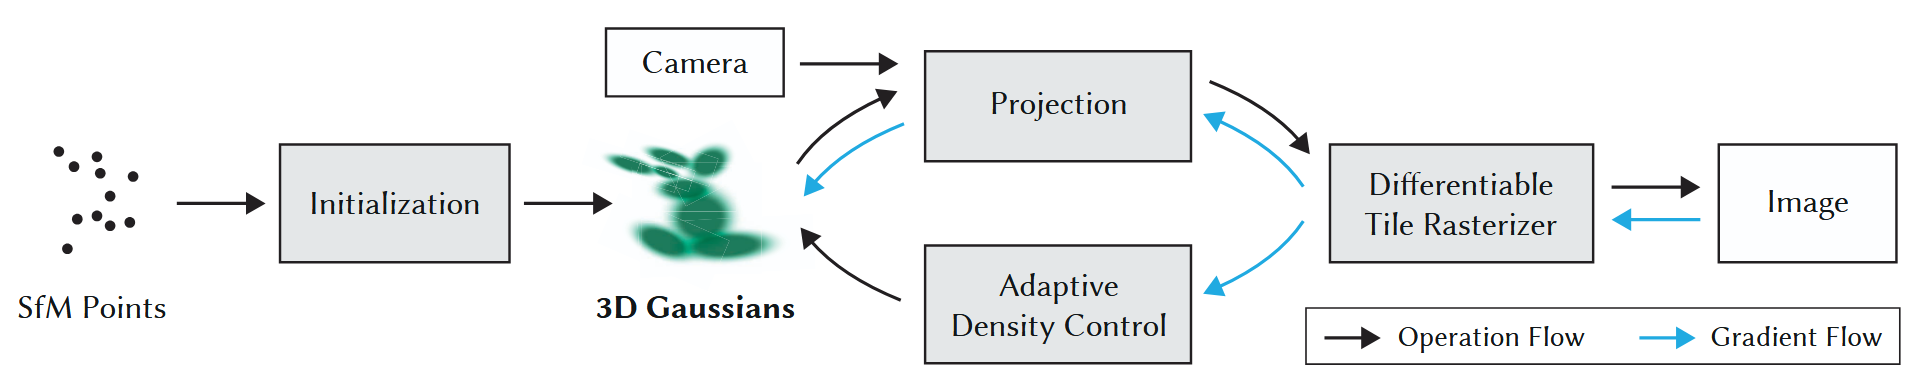
\includegraphics[width=\textwidth]{figuras/kerbl2023_fig2.png}}
    \caption{Visão geral do pipeline do 3D-GS, desde a inicialização com pontos de SfM até a projeção, o controle adaptativo de densidade e a rasterização diferenciável.}
    \label{fig:3dgs_pipeline_kerbl}
    \fonte{Adaptado de \cite{kerbl2023}.}
\end{figure}

Esse mecanismo também introduz desafios: cenas extensas ou detalhadas podem exigir milhões de gaussianas, elevando armazenamento, largura de banda e memória de vídeo \cite{fei2025survey3dgs,chen2024survey3dgs,liu2024citygaussian}. Assim, parte do gargalo desloca-se da amostragem volumétrica para a organização da representação explícita.

\subsection{Eficiência, memória e variantes recentes}

A literatura recente mostra que o 3D-GS se tornou base para métodos voltados a eficiência, compressão, escalabilidade e adaptação a plataformas restritas. Embora a rasterização de gaussianas ofereça desempenho elevado, a representação pode se tornar pesada em memória e sensível à quantidade de primitivas necessárias para preservar detalhes \cite{fei2025survey3dgs,chen2024survey3dgs,wu2025,fang2024}.

Entre as estratégias propostas, destacam-se compressão e poda para reduzir o número de gaussianas ou compactar atributos sem degradar significativamente a qualidade visual. O LightGaussian explora poda, redução de harmônicos esféricos, quantização e armazenamento eficiente \cite{fan2024lightgaussian,fei2025survey3dgs}; outros trabalhos reforçam que o \textit{footprint} de memória é um gargalo para dispositivos limitados \cite{fang2024,huang2025,wu2025}.

Outra direção envolve estruturas hierárquicas, ancoragem e níveis de detalhe. O Scaffold-GS organiza gaussianas a partir de pontos-âncora para reduzir redundâncias \cite{lu2024scaffoldgs}, enquanto abordagens como CityGaussian indicam a necessidade de divisão espacial e controle de nível de detalhe em ambientes grandes \cite{liu2024citygaussian,fei2025survey3dgs}.

Além da memória, a projeção e a composição podem introduzir aliasing, artefatos de ordenação, \textit{floaters} e instabilidades visuais, sobretudo com movimento contínuo de câmera ou detalhes finos \cite{fei2025survey3dgs,chen2024survey3dgs}. Em aplicações imersivas, essas inconsistências podem se tornar mais perceptíveis durante movimentos de cabeça e renderização estereoscópica \cite{xu2023,tu2025}.

O Quadro \ref{qua:comparacao_metodos_3dgs} sintetiza métodos relevantes para a passagem de representações implícitas ou híbridas a estruturas mais adequadas à visualização interativa \cite{mildenhall2020,kerbl2023,chen2024survey3dgs}.

\begin{quadro}[H]
\centering
\footnotesize
\caption{Comparação entre métodos relevantes para síntese de novas vistas e execução interativa.}
\label{qua:comparacao_metodos_3dgs}
\renewcommand{\arraystretch}{1.2}
\setlength{\tabcolsep}{3pt}
\begin{tabularx}{\textwidth}{|p{2.2cm}|p{2.2cm}|p{3.2cm}|p{3.4cm}|X|}
\hline
\textbf{Método} & \textbf{Paradigma} & \textbf{Vantagem principal} & \textbf{Limitação principal} & \textbf{Relação com este trabalho} \\
\hline
NeRF & Implícito & Alta fidelidade visual e representação contínua da cena & Alto custo de inferência por renderização volumétrica & Serve como linha de base conceitual e técnica para reconstrução de cenas estáticas \\
\hline
Instant-NGP & Híbrido / implícito acelerado & Redução expressiva do tempo de treinamento por codificação \textit{hash} multirresolução & Ainda depende de renderização volumétrica e consultas ao campo neural & Apoia a discussão sobre aceleração prática de NeRF e viabilidade experimental \\
\hline
SNeRG / PlenOctrees & Explícito após \textit{baking} & Aproxima campos neurais de representações renderizáveis em tempo real & Exige conversão ou pré-processamento da representação & Mostra a tendência de explicitar representações para visualização interativa \\
\hline
3D-GS & Explícito & Alta qualidade visual com renderização em tempo real por rasterização diferenciável & Alto consumo de memória e sensibilidade à organização das gaussianas & Representação principal considerada para execução interativa em VR \\
\hline
Scaffold-GS / LightGaussian & Explícito otimizado & Redução de redundância, compressão e melhor uso de memória & Maior complexidade de treinamento e possível perda visual se comprimido em excesso & Indica caminhos para adequar 3D-GS a hardware autônomo e restrito \\
\hline
\end{tabularx}
\fonte{Elaboração própria com base em \cite{mildenhall2020,muller2022,yu2021plenoctrees,hedman2021snerg,kerbl2023,lu2024scaffoldgs,fan2024lightgaussian,fei2025survey3dgs}.}
\end{quadro}

\subsection{Relação com Realidade Virtual e com o escopo deste trabalho}

Em Realidade Virtual, a vantagem de renderização do 3D-GS torna-se especialmente relevante, pois aplicações imersivas exigem renderização estereoscópica, baixa latência e estabilidade durante movimentos de cabeça. A literatura de VR-NeRF mostra que mesmo abordagens baseadas em NeRF precisam combinar captura multivista densa, representação eficiente, nível de detalhe e renderização otimizada para alcançar taxas interativas \cite{xu2023}, reforçando o interesse por representações próximas do pipeline gráfico \cite{kerbl2023,tu2025}.

Ainda assim, a adoção de 3D-GS em VR autônoma não é direta. Dispositivos móveis impõem restrições de memória, consumo energético, largura de banda e processamento gráfico; por isso, compressão, poda, seleção de nível de detalhe, renderização foveada e controle de artefatos tornam-se componentes do problema \cite{metaquest3s2024,qualcommxr2gen2,tu2025,fan2024lightgaussian,huang2025}.

Neste trabalho, o 3D-GS é compreendido como mudança de paradigma representacional: a reconstrução inicial pode se apoiar em NeRF ou métodos derivados, enquanto a visualização interativa demanda uma estrutura explícita compatível com rasterização \cite{mildenhall2020,muller2022,kerbl2023}. Essa passagem pode envolver reotimização a partir das mesmas imagens, inicialização por SfM, \textit{baking}, destilação ou outras formas de transição \cite{yu2021plenoctrees,hedman2021snerg,kerbl2023,fei2025survey3dgs}.

Dessa forma, o 3D-GS fornece a base teórica para transformar uma cena reconstruída em ativo visual executável, mas suas limitações de memória, estabilidade perceptual e escalabilidade exigem avaliação específica em VR autônoma \cite{kerbl2023,xu2023,tu2025,metaquest3s2024,qualcommxr2gen2}.

\section{NeRF e 3D-GS como Representações Complementares}

Embora frequentemente apresentados como abordagens concorrentes, NeRF e 3D-GS podem ser compreendidos como representações complementares. O NeRF se destaca por sua natureza implícita e contínua, enquanto o 3D-GS se destaca por primitivas gaussianas rasterizáveis e desempenho de renderização \cite{sitzmann2019srn,mildenhall2020,muller2022,kerbl2023,fei2025survey3dgs}.

Essa complementaridade sustenta a lógica do trabalho: uma representação implícita serve como referência de reconstrução, enquanto uma explícita favorece a execução interativa em VR.

A Figura \ref{fig:nerf_vs_3dgs} sintetiza a passagem de um modelo baseado em amostragem volumétrica para uma estrutura projetável e rasterizável \cite{muller2022,yu2021plenoctrees,hedman2021snerg,kerbl2023,xu2023,tu2025}.

\begin{figure}[H]
    \centering
    \fbox{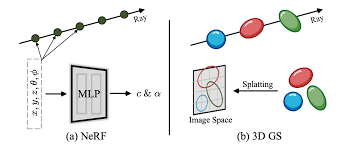
\includegraphics[width=0.72\textwidth]{figuras/nerf_vs_3dgs.png}}
    \caption{Comparação conceitual entre NeRF e 3D Gaussian Splatting. Enquanto o NeRF modela a cena por amostragem ao longo do raio e inferência volumétrica, o 3D-GS representa a cena por gaussianas explícitas projetadas e compostas no plano da imagem.}
    \label{fig:nerf_vs_3dgs}
    \fonte{Adaptado de \cite{chen2024survey3dgs}.}
\end{figure}

Essa relação evidencia um \textit{trade-off}: representações implícitas favorecem continuidade, mas dependem de renderização volumétrica; representações explícitas favorecem velocidade e integração gráfica, mas aumentam exigências de memória, largura de banda e gerenciamento da cena \cite{mildenhall2020,muller2022,kerbl2023,fei2025survey3dgs,fan2024lightgaussian}. O objetivo é compreender como essas características podem ser articuladas em VR autônoma \cite{xu2023,tu2025,metaquest3s2024,qualcommxr2gen2}.

\section{Restrições da Realidade Virtual em Dispositivos Autônomos}

A aplicação de síntese de novas vistas em Realidade Virtual (VR) impõe requisitos mais severos que a visualização convencional. A imagem precisa ser gerada de forma estereoscópica, com alta frequência de atualização e baixa latência, preservando conforto visual, presença e continuidade perceptual durante movimentos de cabeça \cite{xu2023,tu2025}. Quedas de quadros, atraso na pose ou inconsistências entre vistas podem comprometer a fluidez da experiência \cite{xu2023,metaquest3s2024}.

Em dispositivos autônomos, essas restrições são ampliadas por limites de processamento gráfico, memória, consumo energético e dissipação térmica. Métodos custosos em desktop tornam-se mais desafiadores no contexto \textit{on-device}, sobretudo quando exigem renderização estereoscópica em tempo real \cite{metaquest3s2024,qualcommxr2gen2,xu2023}. O VR-NeRF ilustra esse cenário ao demonstrar alto potencial visual em espaços caminháveis, mas também dependência de infraestrutura computacional robusta \cite{xu2023}.

Em representações baseadas em NeRF, o principal desafio decorre da renderização volumétrica, que exige múltiplas amostragens por raio e consultas sucessivas ao campo neural. Esse processo é oneroso em resoluções elevadas, múltiplas vistas e taxas de atualização compatíveis com VR \cite{mildenhall2020,muller2022,xu2023}; por isso, mesmo variantes aceleradas, como Instant-NGP, exigem cautela em hardware autônomo \cite{muller2022,xu2023}.

O 3D Gaussian Splatting substitui a amostragem volumétrica densa por gaussianas projetáveis e rasterizáveis, aproximando-se de pipelines gráficos explorados por GPUs \cite{kerbl2023,fei2025survey3dgs,chen2024survey3dgs}. Entretanto, cenas complexas podem exigir muitas gaussianas, elevando consumo de memória, largura de banda e complexidade de gerenciamento \cite{fei2025survey3dgs,wu2025,fang2024,huang2025,fan2024lightgaussian}.

Assim, a reconstrução visualmente convincente não é suficiente: a representação final precisa ser compatível com execução interativa. Isso exige considerar redução de gaussianas, poda, compressão, seleção de nível de detalhe, \textit{culling} e integração adequada ao motor gráfico \cite{kerbl2023,lu2024scaffoldgs,fan2024lightgaussian,fei2025survey3dgs}, pois o modelo compete por recursos com rastreamento, renderização estereoscópica e demais componentes da aplicação \cite{metaquest3s2024,qualcommxr2gen2,tu2025}.

Além do desempenho bruto, a estabilidade visual também precisa ser considerada. Em VR, artefatos pouco perceptíveis em monitor podem se tornar evidentes pelo campo de visão ampliado e pela movimentação contínua da cabeça. No 3D-GS, \textit{floaters}, aliasing, instabilidades de profundidade e inconsistências entre vistas podem afetar a percepção espacial \cite{kerbl2023,fei2025survey3dgs,chen2024survey3dgs,tu2025}.

Por isso, a avaliação deve observar tanto a qualidade visual, por métricas como PSNR, SSIM e LPIPS \cite{wang2004,zhang2018,mildenhall2020,kerbl2023}, quanto o desempenho, por taxa de quadros, tempo de quadro, uso de memória e estabilidade durante a navegação \cite{xu2023,tu2025,metaquest3s2024}.

Assim, as métricas do trabalho precisam capturar tanto a fidelidade da reconstrução quanto a viabilidade de uso interativo em dispositivo autônomo \cite{mildenhall2020,kerbl2023,xu2023,tu2025}.

\section{Métricas de Avaliação de Qualidade Visual e Desempenho}

A análise do pipeline exige observar conjuntamente qualidade visual e desempenho. Métricas apenas visuais não determinam a viabilidade de uma aplicação imersiva, enquanto métricas apenas computacionais não capturam a fidelidade perceptual da reconstrução. Por isso, adotam-se PSNR, SSIM, LPIPS e FPS como métricas principais, em consonância com a literatura de NeRF, 3D Gaussian Splatting e renderização neural em VR \cite{mildenhall2020,kerbl2023,xu2023,fei2025survey3dgs,chen2024survey3dgs}.

PSNR, SSIM e LPIPS comparam imagens sintetizadas e imagens de referência sob perspectivas complementares: erro pixel a pixel, preservação estrutural e similaridade perceptual. Já FPS, tempo de quadro e uso de memória indicam se a representação pode ser executada em contexto interativo, especialmente em dispositivos autônomos de VR \cite{mildenhall2020,kerbl2023,wang2004,zhang2018,xu2023,tu2025,metaquest3s2024}.

\subsection{PSNR}

O \textit{Peak Signal-to-Noise Ratio} (PSNR) é uma métrica derivada do erro quadrático médio entre a imagem sintetizada e a imagem de referência. Em tarefas de síntese de novas vistas, essa métrica é utilizada para quantificar a proximidade numérica entre os valores dos pixels das imagens comparadas, sendo recorrente em avaliações de NeRF, variantes de renderização neural e métodos baseados em 3D-GS \cite{mildenhall2020,barron2021mipnerf,kerbl2023,fei2025survey3dgs}. Sua formulação clássica é:

\begin{equation}
PSNR = 10 \log_{10}\left(\frac{MAX_I^2}{MSE}\right),
\label{eq:psnr}
\end{equation}
\addEquacao{Cálculo do PSNR}{\ref{eq:psnr}}

em que $MAX_I$ representa o valor máximo possível de intensidade do pixel e $MSE$ é o erro quadrático médio entre a imagem sintetizada e a imagem de referência. O $MSE$ pode ser definido como:

\begin{equation}
MSE = \frac{1}{mn}\sum_{i=1}^{m}\sum_{j=1}^{n}
\left[I(i,j) - \hat{I}(i,j)\right]^2,
\label{eq:mse}
\end{equation}
\addEquacao{Erro quadrático médio entre imagem de referência e imagem sintetizada}{\ref{eq:mse}}

em que $I$ representa a imagem de referência, $\hat{I}$ representa a imagem sintetizada, e $m$ e $n$ correspondem às dimensões da imagem. Em geral, valores mais altos de PSNR indicam maior proximidade entre reconstrução e referência. No entanto, sua interpretação deve ser feita com cautela, pois pequenas variações numéricas nem sempre correspondem diretamente à percepção visual humana, especialmente em cenas com texturas complexas, reflexos ou pequenas diferenças estruturais \cite{mildenhall2020,kerbl2023,zhang2018}.

\subsection{SSIM}

O \textit{Structural Similarity Index Measure} (SSIM) foi proposto para aproximar melhor a percepção humana ao comparar duas imagens em termos de luminância, contraste e estrutura. Diferentemente de métricas baseadas apenas em erro pixel a pixel, o SSIM considera estatísticas locais da imagem, sendo útil para avaliar se a reconstrução preserva formas, bordas e organização estrutural da cena \cite{wang2004,mildenhall2020,kerbl2023}. Sua forma clássica é:

\begin{equation}
SSIM(x,y)=
\frac{(2\mu_x\mu_y + C_1)(2\sigma_{xy}+C_2)}
{(\mu_x^2+\mu_y^2+C_1)(\sigma_x^2+\sigma_y^2+C_2)},
\label{eq:ssim}
\end{equation}
\addEquacao{Cálculo do SSIM}{\ref{eq:ssim}}

em que $\mu_x$ e $\mu_y$ são as médias locais das imagens comparadas, $\sigma_x^2$ e $\sigma_y^2$ são suas variâncias, $\sigma_{xy}$ é a covariância entre elas e $C_1$, $C_2$ são constantes de estabilização. Em síntese de novas vistas, o SSIM complementa o PSNR por penalizar distorções estruturais que podem não gerar grande erro absoluto, mas que afetam a coerência visual da cena reconstruída \cite{wang2004,mildenhall2020,kerbl2023}.

No contexto deste trabalho, o SSIM é relevante por observar estruturas visuais importantes para a percepção espacial \cite{wang2004,xu2023,tu2025}.

\subsection{LPIPS}

O \textit{Learned Perceptual Image Patch Similarity} (LPIPS) mede a distância perceptiva entre duas imagens utilizando ativações internas de redes neurais profundas treinadas para tarefas de visão computacional. Em vez de se basear apenas na diferença direta entre pixels, a métrica compara representações de mais alto nível, associadas a textura, contornos e padrões perceptivos \cite{zhang2018}. Na prática, valores menores de LPIPS indicam maior similaridade perceptual entre a imagem sintetizada e a imagem de referência.

Em síntese de novas vistas, o LPIPS complementa PSNR e SSIM porque diferenças geométricas, texturais ou fotométricas nem sempre são bem capturadas por métricas de erro pixel a pixel. Assim, contribui para uma avaliação mais equilibrada entre fidelidade numérica, preservação estrutural e qualidade perceptual \cite{mildenhall2020,kerbl2023,zhang2018,fei2025survey3dgs}.

\subsection{FPS, tempo de quadro e uso de memória}

Enquanto PSNR, SSIM e LPIPS avaliam qualidade visual, a taxa de quadros por segundo (FPS) e o tempo de renderização por quadro avaliam a fluidez interativa. Em VR, esses indicadores são críticos porque a renderização deve acompanhar os movimentos do usuário, atualizar as duas vistas estereoscópicas e reduzir atrasos perceptíveis \cite{xu2023,tu2025,metaquest3s2024}.

O tempo médio por quadro pode ser relacionado ao FPS pela seguinte expressão:

\begin{equation}
t_{quadro} = \frac{1000}{FPS},
\label{eq:tempo_quadro}
\end{equation}
\addEquacao{Tempo médio de renderização por quadro em milissegundos}{\ref{eq:tempo_quadro}}

em que $t_{quadro}$ é medido em milissegundos. Essa relação indica o custo temporal de renderização: quanto maior o FPS, menor o tempo disponível para gerar cada quadro. Em VR, esse limite é mais restritivo porque cada quadro precisa refletir a pose atualizada do usuário \cite{xu2023,tu2025}.

Além da taxa de quadros, o uso de memória é relevante, sobretudo em representações explícitas como 3D-GS. Número de gaussianas, atributos armazenados, grau dos harmônicos esféricos e organização espacial impactam a viabilidade em plataformas móveis \cite{kerbl2023,fei2025survey3dgs,wu2025,fang2024,huang2025,fan2024lightgaussian}. Por isso, FPS deve ser observado em conjunto com tempo de quadro, consumo de memória e estabilidade.

Em dispositivos autônomos, o desempenho também deve ser interpretado à luz das restrições de energia, dissipação térmica e capacidade gráfica, pois rastreamento, renderização estereoscópica, aplicação e sistema compartilham recursos \cite{metaquest3s2024,qualcommxr2gen2,xu2023}.

Desse modo, as métricas adotadas cobrem duas dimensões complementares: qualidade da reconstrução e viabilidade prática da visualização interativa em VR \cite{mildenhall2020,wang2004,zhang2018,kerbl2023,xu2023,tu2025,metaquest3s2024}.

\section{Meta Quest 3S como Plataforma-Alvo}
\label{sec:meta_quest_3s}

Como o hardware-alvo deste trabalho é o Meta Quest 3S, suas características técnicas influenciam diretamente a viabilidade da visualização imersiva proposta. Em VR autônoma, o headset atua como dispositivo de exibição, plataforma de processamento gráfico, sistema de rastreamento e interface de interação \cite{metaquest3s2024,qualcommxr2gen2,xu2023,tu2025}.

Essa condição difere de uma estação de trabalho com GPU dedicada: no Meta Quest 3S, processamento gráfico, rastreamento, composição estereoscópica, lógica da aplicação e \textit{runtime} XR compartilham os mesmos recursos. A avaliação torna-se mais próxima de um cenário real de uso, mas também mais restritiva \cite{metaquest3s2024,qualcommxr2gen2,xu2023}.

\subsection{Características técnicas do Meta Quest 3S}

Segundo a documentação oficial da Meta, o Meta Quest 3S é um dispositivo \textit{wireless all-in-one} com painel LCD, resolução de 1832$\times$1920 pixels por olho, 20 PPD, taxa de atualização de até 120 Hz, 8 GB de memória embarcada, chipset Snapdragon XR2 Gen 2B, rastreamento de cabeça e mãos, \textit{passthrough} colorido estereoscópico e campo de visão aproximado de 96$^\circ$ na horizontal e 90$^\circ$ na vertical. A plataforma também oferece suporte ao Meta Quest Link \cite{metaquest3s2024}, situando-se como headset móvel moderno, porém sujeito a limites de processamento, memória e dissipação térmica \cite{qualcommxr2gen2,metaquest3s2024}.

\begin{quadro}[H]
\centering
\footnotesize
\caption{Características técnicas relevantes do Meta Quest 3S para o pipeline proposto.}
\label{qua:meta_quest_3s_specs}
\renewcommand{\arraystretch}{1.2}
\setlength{\tabcolsep}{4pt}
\begin{tabularx}{\textwidth}{|p{4.2cm}|X|}
\hline
\textbf{Característica} & \textbf{Implicação para o trabalho} \\
\hline
Resolução de 1832$\times$1920 pixels por olho & Aumenta a demanda de preenchimento de pixels e reforça a necessidade de renderização eficiente em duas vistas estereoscópicas. \\
\hline
Taxa de atualização de até 120 Hz & Define uma referência de fluidez para aplicações imersivas, exigindo baixo tempo de renderização por quadro. \\
\hline
8 GB de memória embarcada & Limita o tamanho prático das representações explícitas, especialmente em modelos 3D-GS com grande número de gaussianas. \\
\hline
Snapdragon XR2 Gen 2B & Indica uma plataforma móvel de XR, com capacidade gráfica integrada e orçamento computacional inferior ao de GPUs desktop dedicadas. \\
\hline
Rastreamento de cabeça e mãos & Exige que a aplicação responda continuamente à pose do usuário, tornando quedas de desempenho mais perceptíveis. \\
\hline
\textit{Passthrough} colorido estereoscópico & Amplia possibilidades de aplicações imersivas e mistas, mas também compete por recursos do sistema. \\
\hline
Suporte ao Meta Quest Link & Permite comparação entre execução autônoma e execução conectada a um computador, funcionando como alternativa metodológica de contingência. \\
\hline
\end{tabularx}
\fonte{Elaboração própria com base em \cite{metaquest3s2024,qualcommxr2gen2}.}
\end{quadro}

Essas especificações reforçam que o Quest 3S é adequado como plataforma experimental por combinar recursos contemporâneos de interação e visualização com orçamento computacional móvel. Portanto, a avaliação deve considerar não apenas fidelidade visual, mas também custo prático de execução \cite{metaquest3s2024,qualcommxr2gen2,xu2023,tu2025}.

Do ponto de vista comparativo, a documentação oficial indica que o Quest 3S compartilha com o Quest 3 a mesma classe de chipset e a mesma quantidade de memória, embora tenha resolução e campo de visão mais modestos. Essa combinação delimita experimentalmente o problema e evita uma análise restrita a condições ideais de hardware desktop \cite{metaquest3s2024,qualcommxr2gen2}.

\subsection{Implicações do hardware para NeRF e 3D Gaussian Splatting}

A adoção do Meta Quest 3S afeta diretamente a escolha da representação visual e a avaliação da solução. Embora o NeRF ofereça elevada fidelidade, sua formulação volumétrica é onerosa para execução \textit{on-device}, especialmente com renderização estereoscópica e atualização em alta frequência \cite{mildenhall2020,muller2022,xu2023,metaquest3s2024}.

Nesse cenário, o Quest 3S reforça a motivação para investigar representações explícitas. O 3D Gaussian Splatting dispensa amostragem densa ao longo do raio e se apoia em rasterização diferenciável \cite{kerbl2023,fei2025survey3dgs,chen2024survey3dgs}, mas número de gaussianas, largura de banda e memória continuam críticos em cenas complexas \cite{wu2025,fang2024,huang2025,fan2024lightgaussian}.

O suporte a até 120 Hz deve ser entendido como referência de exigência, não como garantia de desempenho. Em aplicações imersivas, estabilidade da taxa de quadros e previsibilidade do tempo de renderização são tão importantes quanto a qualidade visual. Trabalhos como VR-NeRF evidenciam a pressão imposta por resolução por olho, renderização estereoscópica e fluidez \cite{xu2023}, especialmente quando se busca execução autônoma \cite{metaquest3s2024,qualcommxr2gen2,tu2025}.

Portanto, a adequação ao Quest 3S depende de observar se a cena mantém qualidade visual, estabilidade e consumo de memória compatíveis com uma aplicação imersiva real, possivelmente exigindo compressão, poda, hierarquização, seleção de nível de detalhe e organização espacial \cite{lu2024scaffoldgs,fan2024lightgaussian,fei2025survey3dgs,wu2025}.

\subsection{Quest 3S como referência experimental do trabalho}

A escolha do Meta Quest 3S possui relevância metodológica por se tratar de um dispositivo comercial, autônomo e representativo de headsets móveis contemporâneos. Seu uso obriga o pipeline a enfrentar limites reais de memória, renderização estereoscópica, consumo energético, dissipação térmica e sensibilidade a quedas de desempenho \cite{metaquest3s2024,qualcommxr2gen2,xu2023}.

Nesse sentido, o dispositivo funciona como referência concreta para analisar a relação entre qualidade visual, memória, estabilidade e interatividade \cite{mildenhall2020,muller2022,kerbl2023,metaquest3s2024}.

A plataforma também permite diferenciar dois níveis de avaliação: qualidade visual, por PSNR, SSIM e LPIPS \cite{wang2004,zhang2018,mildenhall2020,kerbl2023}, e execução, por FPS, tempo de quadro, uso de memória e estabilidade durante a navegação \cite{xu2023,tu2025,metaquest3s2024}. Essa separação é necessária porque uma representação pode ser visualmente adequada em avaliação offline e ainda assim inadequada para uso interativo.

Por fim, o suporte ao Meta Quest Link preserva uma contingência metodológica: caso a execução nativa seja limitada, a execução conectada ao computador pode servir como referência comparativa entre desempenho \textit{on-device} e desempenho assistido por hardware externo \cite{metaquest3s2024}. A meta principal, entretanto, permanece a avaliação em contexto autônomo.

Uma vez delimitadas as características da plataforma-alvo, torna-se necessário discutir como diferentes \textit{engines} podem mediar a integração entre representação da cena, \textit{runtime} XR e execução prática em VR \cite{jin2024,kerbl2023,tu2025,metaquest3s2024}.

\section{Engines para Integração em Realidade Virtual}

A integração de uma cena reconstruída em um ambiente de Realidade Virtual depende não apenas da representação adotada, mas também da infraestrutura de software responsável por carregar, renderizar, otimizar e executar essa representação no dispositivo-alvo. Nesse contexto, as \textit{engines} gráficas atuam como camadas intermediárias entre os ativos tridimensionais, o \textit{runtime} XR, o sistema de entrada, a câmera estereoscópica e os mecanismos de empacotamento para plataformas móveis, como o Meta Quest 3S \cite{metaquest3s2024,qualcommxr2gen2,xu2023,tu2025}.

No caso de representações neurais ou derivadas, como NeRF e 3D Gaussian Splatting, essa camada de integração torna-se ainda mais relevante. O NeRF depende de renderização volumétrica e múltiplas consultas por raio, enquanto o 3D-GS utiliza primitivas explícitas projetadas e compostas por rasterização diferenciável. Embora o 3D-GS seja mais compatível com renderização interativa, sua execução prática ainda depende de suporte adequado a shaders, estruturas de dados, gerenciamento de memória e integração com o pipeline gráfico da aplicação \cite{mildenhall2020,muller2022,kerbl2023,fei2025survey3dgs,chen2024survey3dgs}.

Do ponto de vista da Fundamentação Teórica, a análise das engines não deve ser compreendida como uma decisão de projeto, mas como uma caracterização das possibilidades técnicas disponíveis para integração em VR. A escolha específica da engine, bem como a justificativa metodológica dessa escolha, pertence ao capítulo de Projeto, no qual são definidas as decisões de implementação, os riscos assumidos e as estratégias de contingência. Nesta seção, portanto, descrevem-se apenas os critérios gerais e as principais alternativas de integração.

\subsection{Critérios de caracterização das engines}

Uma engine voltada à integração em VR pode ser caracterizada a partir de alguns critérios técnicos recorrentes. O primeiro é a maturidade do suporte a XR, incluindo câmera estereoscópica, rastreamento de cabeça e mãos, entrada por controladores, suporte a OpenXR e empacotamento para dispositivos autônomos. O segundo é a capacidade de otimização gráfica, envolvendo recursos como controle de qualidade visual, \textit{culling}, gerenciamento de memória, renderização em múltiplas vistas e adaptação a GPUs móveis \cite{xu2023,tu2025,metaquest3s2024}.

O terceiro critério diz respeito à flexibilidade de integração com representações não convencionais, como 3D Gaussian Splatting. Diferentemente de malhas triangulares tradicionais, modelos 3D-GS exigem rotinas específicas para armazenamento, ordenação, projeção e composição de gaussianas. Por isso, a engine precisa permitir a implementação ou adaptação de renderizadores, shaders, plugins e formatos de importação compatíveis com esse tipo de representação \cite{kerbl2023,jin2024,fei2025survey3dgs,chen2024survey3dgs}.

O quarto critério é a previsibilidade do ciclo de desenvolvimento. Em aplicações para headsets autônomos, a viabilidade experimental depende de um fluxo confiável de testes, geração de \textit{builds}, depuração no dispositivo e coleta de métricas. Como o desempenho final observado em VR resulta da interação entre representação, engine, runtime XR e hardware, a escolha da ferramenta de integração afeta diretamente a interpretação dos resultados experimentais \cite{xu2023,tu2025,metaquest3s2024}.

\subsection{Unreal Engine}

A Unreal Engine é uma engine amplamente utilizada em aplicações gráficas de alta fidelidade, simulação e experiências imersivas. Sua arquitetura oferece suporte a renderização em tempo real, recursos avançados de gerenciamento de cena, integração com XR e mecanismos de empacotamento para diferentes plataformas. Em contextos de VR, essas características são relevantes porque a aplicação precisa coordenar renderização estereoscópica, entrada do usuário, atualização de pose e desempenho estável em tempo real \cite{xu2023,tu2025,metaquest3s2024}.

No contexto específico de 3D Gaussian Splatting, a literatura recente já apresenta esforços de integração dessa representação à Unreal Engine. O UE-GS, por exemplo, investiga a integração de 3D-GS ao ambiente da Unreal, evidenciando a possibilidade de aproximar modelos gaussianos explícitos de um pipeline de renderização usado em aplicações interativas \cite{jin2024}. Essa relação torna a Unreal uma alternativa relevante para estudos que buscam conectar representações derivadas de reconstrução neural a ambientes imersivos.

Por outro lado, a Unreal Engine também apresenta maior complexidade de configuração e integração quando comparada a fluxos mais simples de prototipagem. A combinação entre versões do motor, plugins experimentais, formatos específicos de importação, shaders personalizados e geração de \textit{builds} para dispositivos Quest pode introduzir riscos técnicos \cite{jin2024,kerbl2023,fei2025survey3dgs,metaquest3s2024}.

\subsection{Unity}

A Unity é uma engine frequentemente associada a fluxos de prototipagem rápida, aplicações interativas e desenvolvimento multiplataforma. Em projetos de VR, sua relevância decorre da disponibilidade de ferramentas voltadas à criação de cenas interativas, manipulação de objetos, integração com dispositivos XR e ciclos iterativos de teste. Em cenários acadêmicos e experimentais, essas características podem facilitar a construção de protótipos funcionais e a validação inicial de interações em headset \cite{xu2023,tu2025,metaquest3s2024}.

Para aplicações baseadas em 3D Gaussian Splatting, a Unity pode ser analisada como uma alternativa de integração quando o objetivo é observar o comportamento de uma representação explícita em uma aplicação XR. Entretanto, assim como em outras engines generalistas, a adoção de 3D-GS exige algum nível de adaptação do pipeline convencional, pois a representação por gaussianas não corresponde diretamente aos formatos tradicionais de malhas, materiais e texturas \cite{kerbl2023,fei2025survey3dgs,chen2024survey3dgs}.

Dessa forma, a caracterização da Unity deve considerar dois aspectos simultâneos: por um lado, sua utilidade em fluxos iterativos e aplicações XR; por outro, a necessidade de adaptação para lidar com representações gaussianas especializadas \cite{xu2023,tu2025,metaquest3s2024}.

\subsection{Godot}

A Godot representa uma alternativa de engine aberta e flexível, com possibilidade de customização do fluxo de desenvolvimento e menor dependência de ecossistemas proprietários. Em um contexto acadêmico, engines abertas podem ser relevantes por favorecerem experimentação, inspeção do funcionamento interno e adaptação de partes específicas do pipeline de renderização \cite{tu2025,kerbl2023,fei2025survey3dgs}.

Entretanto, quando o objetivo envolve integração de 3D Gaussian Splatting, execução em headset autônomo e análise de desempenho em VR, a maturidade do ecossistema e a disponibilidade de fluxos já validados tornam-se aspectos importantes. Como o 3D-GS exige rotinas específicas de projeção, composição, gerenciamento de memória e atualização em tempo real, engines com menor quantidade de referências consolidadas para esse caso de uso podem demandar maior esforço de implementação experimental \cite{kerbl2023,fei2025survey3dgs,chen2024survey3dgs,metaquest3s2024}.

Assim, a Godot pode ser descrita como uma possibilidade de experimentação e customização, especialmente em estudos interessados em maior controle sobre o pipeline. Contudo, sua caracterização teórica deve reconhecer que a integração de representações especializadas em VR autônoma depende não apenas da abertura da engine, mas também da disponibilidade de ferramentas, plugins, documentação, suporte XR e mecanismos de otimização adequados ao dispositivo-alvo \cite{xu2023,tu2025,metaquest3s2024}.

\subsection{Visualizadores dedicados e execução assistida por desktop}

Além das engines generalistas, outra possibilidade de integração consiste no uso de visualizadores dedicados ou aplicações executadas em ambiente desktop com transmissão para o headset. Essa abordagem é comum em cenários nos quais o objetivo principal é avaliar a visualização imersiva da cena, mas a execução totalmente nativa no dispositivo ainda apresenta restrições de desempenho ou de integração \cite{xu2023,metaquest3s2024}.

Do ponto de vista técnico, a execução assistida por desktop pode aliviar parte da pressão imposta pelo hardware móvel, deslocando o processamento pesado para uma GPU externa. O VR-NeRF demonstra que a renderização neural de alta fidelidade em espaços caminháveis pode demandar infraestrutura computacional substancial, incluindo renderização em resolução elevada, múltiplas vistas e otimizações específicas para VR \cite{xu2023}. Dessa forma, visualizadores dedicados e execução via desktop podem funcionar como referência comparativa para compreender os limites entre visualização imersiva assistida e execução autônoma.

No entanto, essa abordagem não representa o mesmo problema de execução \textit{on-device}. Quando o processamento ocorre em um computador externo, parte das restrições de memória, energia, dissipação térmica e GPU móvel deixa de ser observada diretamente. Por isso, em uma análise experimental, resultados obtidos via desktop ou Quest Link devem ser interpretados como uma condição distinta da execução nativa no headset \cite{metaquest3s2024,qualcommxr2gen2,xu2023}.

\subsection{Síntese descritiva}

O Quadro \ref{qua:comparativo_engines_vr} sintetiza as características gerais das alternativas discutidas. A tabela não estabelece uma escolha de implementação, mas organiza os principais aspectos técnicos que podem orientar a decisão posteriormente no capítulo de Projeto.

\begin{quadro}[H]
\centering
\caption{Síntese descritiva de engines e abordagens para integração em VR}
\label{qua:comparativo_engines_vr}
\footnotesize
\renewcommand{\arraystretch}{1.2}
\begin{tabularx}{\textwidth}{|>{\raggedright\arraybackslash}p{3.2cm}|>{\raggedright\arraybackslash}X|>{\raggedright\arraybackslash}X|}
\hline
\textbf{Engine / abordagem} & \textbf{Características gerais} & \textbf{Pontos de atenção} \\ \hline
Unreal Engine & Engine voltada a aplicações gráficas de alta fidelidade, com suporte a XR, renderização em tempo real e registros recentes de integração com 3D-GS. & Maior complexidade de integração, dependência de plugins, versões do motor, shaders e fluxo de \textit{build} para Quest. \\ \hline
Unity & Engine associada a prototipagem rápida, aplicações interativas e desenvolvimento multiplataforma em XR. & Necessidade de adaptar o pipeline de 3D-GS a formatos, renderizadores e rotinas compatíveis com a engine. \\ \hline
Godot & Engine aberta, flexível e customizável, com interesse acadêmico para experimentação e controle do pipeline. & Menor disponibilidade de fluxos consolidados para 3D-GS em VR autônoma e possível aumento do esforço de implementação. \\ \hline
Visualizador desktop + Quest Link & Execução assistida por desktop com exibição imersiva no headset, útil para comparação com cenários de maior capacidade computacional. & Não representa integralmente a execução \textit{on-device}, pois desloca processamento, memória e carga gráfica para o computador. \\ \hline
\end{tabularx}
\fonte{Elaboração própria com base em \cite{xu2023,kerbl2023,jin2024,tu2025,metaquest3s2024,fei2025survey3dgs}.}
\end{quadro}

A partir dessa síntese, observa-se que cada alternativa oferece possibilidades e limitações distintas para a integração de cenas reconstruídas em VR. Engines generalistas fornecem infraestrutura para interação, câmera estereoscópica, empacotamento e integração com XR, mas podem demandar adaptações específicas para suportar representações como 3D Gaussian Splatting. Visualizadores dedicados, por sua vez, podem simplificar a execução de modelos especializados, mas tendem a reduzir a aderência ao cenário de aplicação autônoma \cite{xu2023,kerbl2023,tu2025,metaquest3s2024}.

\section{Trabalhos relacionados}

A presente seção tem por finalidade situar a proposta desta pesquisa no contexto da produção científica recente sobre representações neurais de cena, com ênfase em \textit{Neural Radiance Fields} (NeRF), \textit{3D Gaussian Splatting} (3DGS) e aplicações voltadas à síntese de novas vistas, renderização em tempo real e realidade virtual. Mais do que apresentar uma enumeração de estudos correlatos, busca-se estabelecer um posicionamento analítico da pesquisa, evidenciando os avanços do estado da arte, as limitações ainda presentes e a lacuna específica à qual esta investigação se vincula.

Para organizar essa análise, os estudos foram selecionados por meio de um protocolo de revisão com foco aplicado, descrito nas subseções seguintes.

\subsection{Protocolo de busca e seleção dos estudos}

O protocolo adotado delimita o objetivo da revisão, a base de busca, o recorte temporal, o idioma, a string utilizada e os critérios de inclusão e exclusão dos estudos. Com isso, busca-se tornar explícito o processo de seleção das referências analisadas e reduzir a subjetividade da revisão.

\subsection{Objetivo da revisão}

O objetivo da revisão foi identificar e analisar estudos que contribuam para a compreensão das seguintes dimensões do problema:

\begin{itemize}
    \item fundamentos das representações implícitas baseadas em NeRF;
    \item técnicas de aceleração da reconstrução e da renderização neural;
    \item alternativas explícitas voltadas ao desempenho em tempo real;
    \item estudos que tratem da adaptação dessas representações ao contexto de realidade virtual;
    \item trabalhos que discutam integração com motores gráficos e ambientes de execução interativos.
\end{itemize}

A revisão foi orientada, portanto, pela seguinte questão de pesquisa:

\begin{quote}
\textit{De que maneira os estudos recentes sobre NeRF e 3D Gaussian Splatting enfrentam o compromisso entre qualidade visual, desempenho computacional e adequação ao uso em aplicações de realidade virtual?}
\end{quote}

\subsection{Base de busca, recorte temporal e idioma}

Como base principal de busca, foi adotado o Google Scholar, em razão de sua abrangência na indexação de artigos de periódicos, anais de conferências e publicações amplamente reconhecidas na área de Computação Gráfica, Visão Computacional e Realidade Virtual. Tal escolha também se mostrou coerente com a orientação de priorizar estudos consolidados e evitar a dependência de versões preliminares disponibilizadas apenas como \textit{preprints}.

O recorte temporal considerado compreende o período de 2020 a 2025. A escolha desse intervalo decorre do fato de que o trabalho seminal sobre NeRF foi publicado em 2020, inaugurando uma nova fase de intensa produção científica em torno de representações neurais para síntese de vistas. A partir de 2023, com a publicação do 3D Gaussian Splatting, observa-se uma inflexão importante na literatura, marcada pela valorização de representações explícitas orientadas ao desempenho em tempo real. O idioma prioritariamente considerado foi o inglês, por concentrar os principais veículos científicos da área.

\subsection{String de busca}

A estratégia de busca foi estruturada a partir de operadores booleanos,
combinando os principais descritores associados ao problema investigado. Uma
forma representativa da string empregada é apresentada a seguir:

\begingroup
\shorthandoff{"}
\begin{quote}
\ttfamily\raggedright
("Neural Radiance Fields" OR NeRF OR "3D Gaussian Splatting") AND ("virtual reality" OR VR OR "real-time rendering" OR "walkable spaces" OR "Unreal Engine")
\end{quote}
\endgroup

Em buscas complementares, foram utilizados termos adicionais, como \texttt{"scene \newline reconstruction"}, \texttt{"novel view synthesis"} e \texttt{"immersive rendering"}, \\ com o objetivo de refinar os resultados e ampliar a aderência ao escopo da pesquisa.

\subsection{Critérios de inclusão e exclusão}

Foram definidos os seguintes critérios de inclusão:

\begin{itemize}
    \item estudos publicados em periódicos ou anais de conferências reconhecidos na área;
    \item estudos publicados entre 2020 e 2025;
    \item pesquisas diretamente associadas a NeRF, 3DGS, reconstrução de cenas, síntese de novas vistas, renderização em tempo real ou realidade virtual;
    \item estudos que apresentem contribuição conceitual, metodológica ou aplicada relevante para o problema de pesquisa do presente trabalho.
\end{itemize}

Por sua vez, os critérios de exclusão foram:

\begin{itemize}
    \item estudos disponíveis apenas em versões preliminares, sem publicação formal consolidada;
    \item estudos sem aderência direta ao tema de reconstrução de cenas e visualização imersiva;
    \item publicações duplicadas ou versões redundantes de um mesmo trabalho;
    \item artigos cujo foco principal se situe em problemas periféricos ao escopo desta pesquisa.
\end{itemize}

\section{Discussão dos estudos selecionados}

Esta seção discute os estudos selecionados, destacando suas principais contribuições, limitações e relações com o \textit{pipeline} proposto nesta pesquisa.

\subsection{\textit{NeRF: Representing Scenes as Neural Radiance Fields for View Synthesis}}

O trabalho de Mildenhall et al. \cite{mildenhall2020} constitui o marco fundador da linha contemporânea de pesquisa em campos neurais para síntese de novas vistas.

Sua principal contribuição está na formulação de uma representação implícita contínua da cena, parametrizada por uma rede neural do tipo \textit{multilayer perceptron} (MLP), que recebe como entrada uma coordenada espacial tridimensional e uma direção de observação, produzindo como saída a densidade volumétrica e a cor correspondente naquele ponto. A imagem final é obtida por integração ao longo dos raios emitidos pela câmera, em um processo de renderização volumétrica diferenciável.

A Figura \ref{fig:nerf_esquema} é especialmente elucidativa porque condensa, em um único diagrama, o núcleo conceitual do método. Observa-se que o modelo não aprende diretamente uma malha, uma nuvem de pontos ou uma textura, mas sim uma função contínua que associa amostras espaciais a propriedades radiométricas. Esse aspecto é decisivo para compreender tanto a capacidade do NeRF de produzir vistas fotorealistas quanto seu custo computacional: como a imagem precisa ser composta a partir de múltiplas amostras por raio, a elevada fidelidade visual vem acompanhada de um processo de inferência oneroso.

\begin{figure}[H]
    \centering
    \fbox{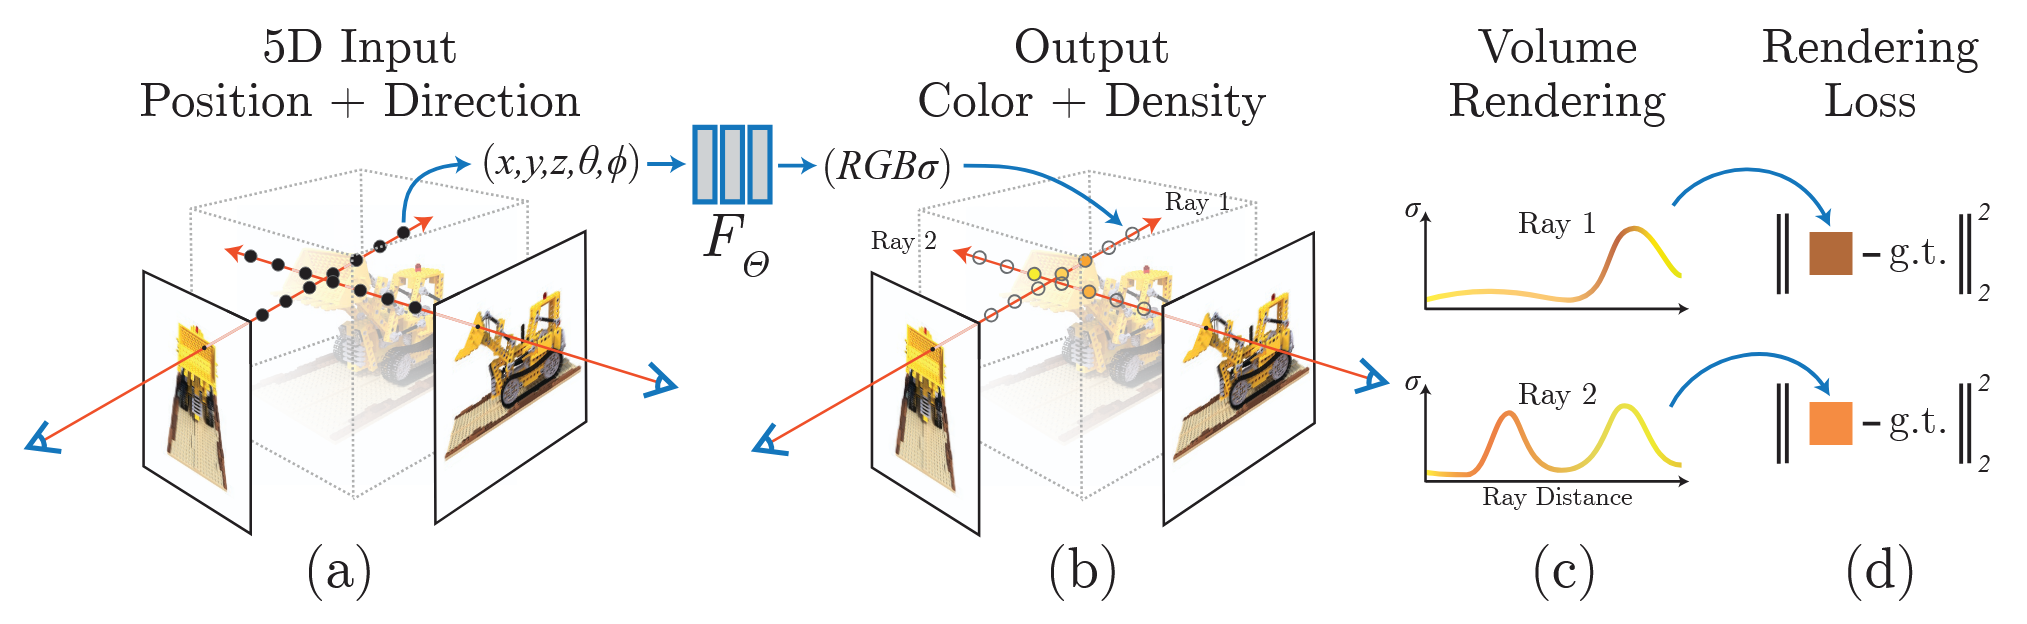
\includegraphics[width=0.92\textwidth]{figuras/mildenhall2020_fig2.png}}
    \caption{Representação esquemática do NeRF. A figura mostra a entrada 5D composta por posição e direção de observação, o mapeamento por uma MLP para cor e densidade e, por fim, a integração volumétrica ao longo dos raios. Fonte: \cite{mildenhall2020}.}
    \label{fig:nerf_esquema}
\end{figure}

Essa formulação foi decisiva porque rompeu com abordagens anteriores baseadas em discretizações rígidas, voxels densos ou estruturas explícitas de custo elevado, oferecendo uma representação compacta e contínua, capaz de modelar efeitos dependentes da direção de observação e detalhes geométricos complexos. O artigo demonstra que, a partir de um conjunto relativamente esparso de imagens com poses conhecidas, é possível sintetizar novas vistas com alto grau de fotorrealismo e consistência multivista.

Para a presente pesquisa, este trabalho é central porque estabelece o referencial teórico a partir do qual se desenvolvem tanto as técnicas de aceleração quanto as alternativas explícitas posteriormente discutidas. Ao mesmo tempo, ele explicita uma limitação estrutural importante: a elevada demanda computacional associada ao treinamento e, sobretudo, à renderização baseada em amostragem volumétrica ao longo dos raios. Em consequência, embora o NeRF apresente notável qualidade de reconstrução e síntese, sua aplicação direta em ambientes imersivos em tempo real permanece restrita.

\subsection{\textit{Instant Neural Graphics Primitives with a Multiresolution Hash Encoding}}

Müller et al. \cite{muller2022} propõem uma contribuição decisiva para a viabilidade prática das representações neurais ao introduzir uma estratégia de codificação multirresolução baseada em tabelas hash treináveis. Em vez de depositar toda a capacidade representacional em uma MLP relativamente grande, o método distribui uma parte significativa da descrição espacial da cena em uma estrutura hierárquica de características indexadas de forma eficiente, permitindo o uso de redes menores e uma inferência mais rápida.

A Figura \ref{fig:instantngp_encoding} é particularmente relevante porque não se limita a ilustrar o método, mas demonstra empiricamente por que a codificação proposta se tornou tão influente. A comparação mostra que abordagens sem codificação ou com codificações convencionais tendem a produzir resultados mais borrados ou a exigir estruturas muito mais pesadas. Em contrapartida, a tabela hash multirresolução apresentada pelos autores preserva detalhes finos com um custo computacional mais favorável. Assim, a imagem sustenta visualmente o argumento central do artigo: ganhos expressivos de eficiência podem ser obtidos por meio da representação dos dados, e não apenas pelo aumento da capacidade da rede.

\begin{figure}[H]
    \centering
    \fbox{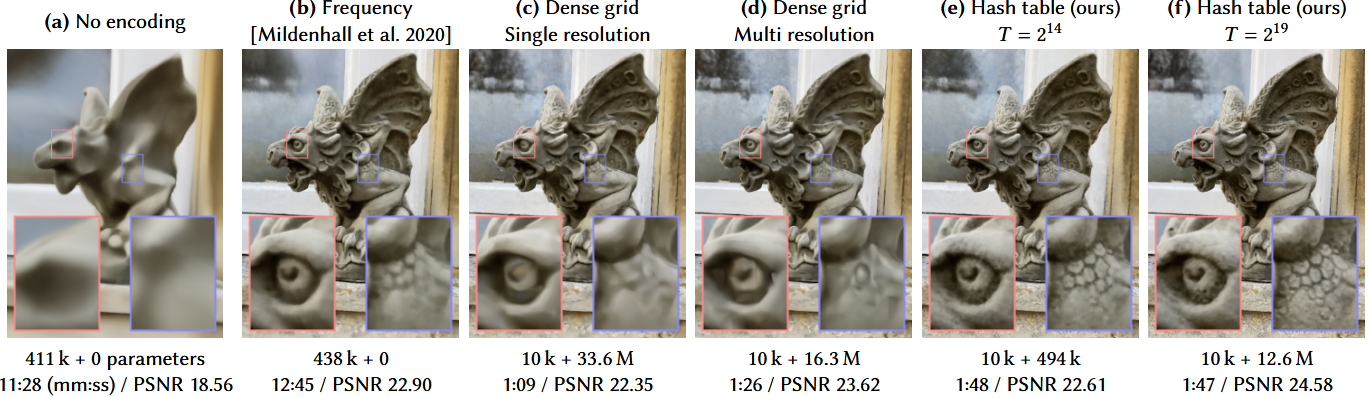
\includegraphics[width=0.95\textwidth]{figuras/muller_fig2.png}}
    \caption{Comparação entre diferentes estratégias de codificação no Instant-NGP. A figura evidencia o compromisso entre número de parâmetros, tempo de treinamento e qualidade visual, destacando o desempenho da codificação por tabela hash multirresolução. Fonte: \cite{muller2022}.}
    \label{fig:instantngp_encoding}
\end{figure}

O avanço apresentado por esse trabalho é particularmente relevante porque atenua uma das principais restrições do NeRF original: o elevado custo de otimização. Ao reduzir drasticamente o tempo necessário para treinamento, o Instant-NGP reposiciona os campos neurais como ferramentas mais acessíveis em contextos experimentais, prototipagem rápida e reconstrução iterativa. Além disso, o método também evidencia que ganhos substanciais de desempenho podem ser obtidos não apenas por mudanças na formulação do modelo, mas sobretudo por escolhas de representação e implementação fortemente alinhadas à arquitetura de hardware disponível.

No contexto desta pesquisa, a relevância do Instant-NGP reside em funcionar como elo intermediário entre a formulação original do NeRF e os esforços posteriores de aproximação ao tempo real. O artigo não elimina integralmente os obstáculos à adoção em realidade virtual, mas demonstra que a fronteira entre qualidade visual e viabilidade computacional é mais flexível do que sugeria a formulação inicial dos campos neurais. Isso é particularmente importante para um trabalho que busca avaliar a aplicabilidade de técnicas neurais em um \textit{pipeline} orientado à visualização imersiva.

Outro aspecto relevante é que o Instant-NGP influenciou diretamente trabalhos posteriores voltados à captura e renderização de cenas complexas, inclusive em contextos de alta resolução e amplo alcance espacial. Assim, mais do que uma técnica de aceleração isolada, o artigo representa uma mudança de perspectiva: ele mostra que a discussão sobre representações neurais de cena deve considerar, simultaneamente, a formulação matemática, a estrutura de dados e a eficiência de execução.

\subsection{\textit{VR-NeRF: High-Fidelity Virtualized Walkable Spaces}}

Xu et al. \cite{xu2023} apresenta um dos trabalhos mais próximos do problema investigado nesta pesquisa, ao propor um sistema de ponta a ponta para captura, reconstrução e visualização de espaços caminháveis em realidade virtual. A contribuição do estudo não se limita à modelagem da cena, mas abrange todo o \textit{pipeline}, desde a aquisição de imagens em alta resolução e alta faixa dinâmica até a renderização em tempo compatível com uma experiência imersiva. Esse caráter sistêmico torna o trabalho particularmente relevante, pois aproxima a discussão acadêmica de um cenário de uso efetivo.

A Figura \ref{fig:vrnerf_overview} evidencia o caráter sistêmico da proposta. Diferentemente de trabalhos centrados apenas na síntese de novas vistas em visualização convencional, o VR-NeRF articula captura especializada, modelagem adaptada e renderização binocular, deixando claro que o problema em VR não se resume à qualidade da reconstrução. A imagem também é relevante por mostrar que os autores tratam explicitamente componentes auxiliares, como profundidade, normais, níveis de detalhe e grade de ocupação, indicando uma preocupação com eficiência e estabilidade visual além da simples reprodução fotográfica.

\begin{figure}[H]
    \centering
    \fbox{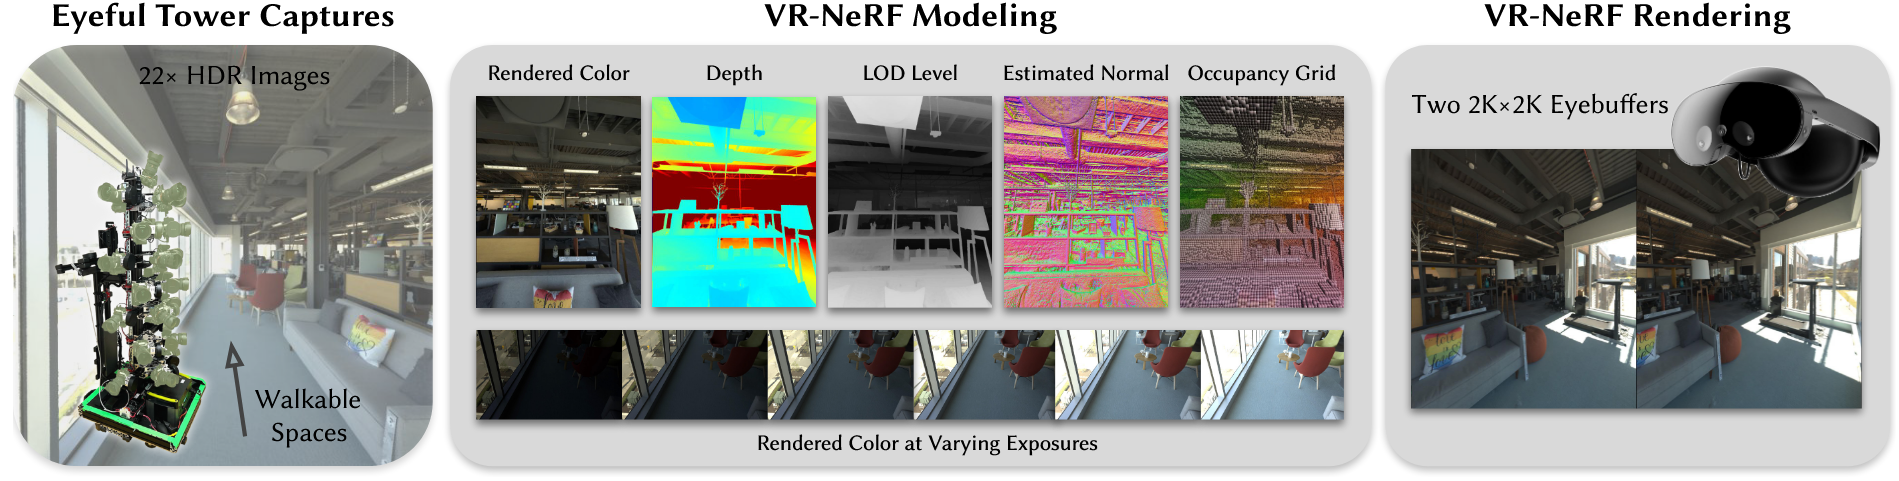
\includegraphics[width=0.98\textwidth]{figuras/xu_2023_fig1.png}}
    \caption{Visão geral do sistema VR-NeRF, contemplando captura, modelagem da cena e renderização em \textit{eyebuffers} binoculares para realidade virtual. Fonte: \cite{xu2023}.}
    \label{fig:vrnerf_overview}
\end{figure}

Um dos diferenciais centrais do VR-NeRF é a preocupação com limitações específicas da realidade virtual. Em vez de tratar o problema apenas como síntese de novas vistas, os autores consideram exigências como liberdade de exploração espacial, estabilidade visual, alta resolução binocular, preservação de detalhes finos e compatibilidade com renderização interativa. Para isso, o trabalho combina adaptações na linha do Instant-NGP, como tratamento mais adequado de imagens HDR, mecanismos de \textit{level of detail} e estratégias de renderização multi-GPU.

A Figura \ref{fig:vrnerf_scaling} complementa a discussão ao tornar visível um dos pontos mais importantes do artigo: a dependência de infraestrutura robusta para alcançar desempenho compatível com VR. As curvas mostram que a taxa de quadros cresce com o número de GPUs, enquanto as linhas de referência tornam explícitos os patamares de desempenho almejados. Em termos analíticos, essa imagem é
fundamental porque reforça uma conclusão importante para a presente pesquisa: o VR-NeRF demonstra a viabilidade técnica da abordagem implícita, mas essa viabilidade ainda se apoia em um orçamento computacional elevado.

\begin{figure}[H]
    \centering
    \fbox{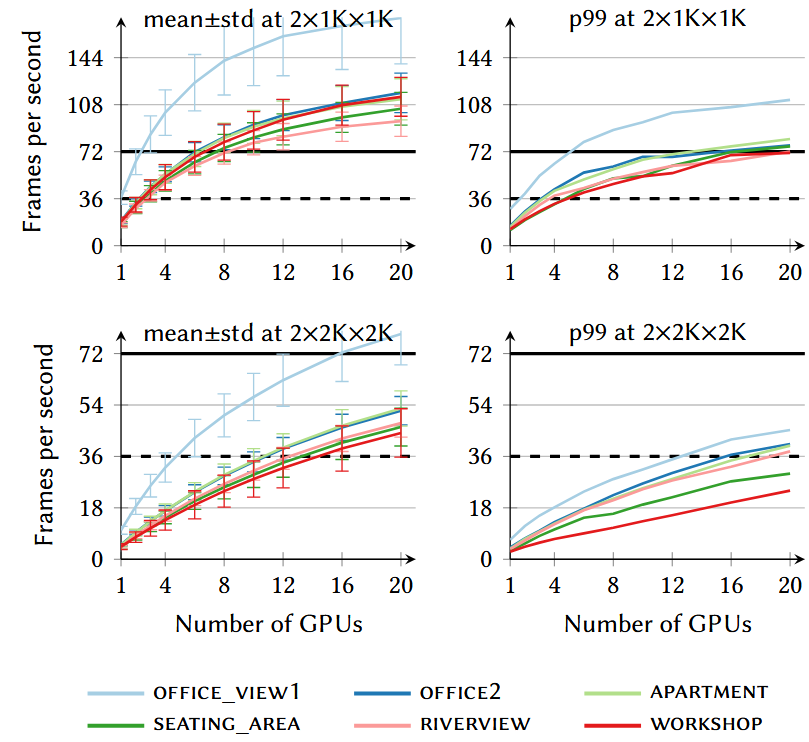
\includegraphics[width=0.72\textwidth]{figuras/xu_2023_fig3.png}}
    \caption{Escalabilidade do VR-NeRF em função do número de GPUs, com indicação dos patamares de desempenho associados à renderização imersiva em diferentes resoluções binoculares. Fonte: \cite{xu2023}.}
    \label{fig:vrnerf_scaling}
\end{figure}

Para o presente trabalho, essa dualidade é especialmente importante. O VR-NeRF funciona como prova de conceito de que campos neurais podem, em condições apropriadas, sustentar experiências imersivas de alta fidelidade. Contudo, também expõe a necessidade de investigar soluções mais pragmáticas, seja por meio de representações mais leves, seja pela conversão para estruturas explícitas mais compatíveis com a renderização em tempo real. Dessa forma, o artigo serve como referência de alto nível para delimitar tanto o potencial quanto as limitações da linha implícita em aplicações de VR.

\subsection{\textit{3D Gaussian Splatting for Real-Time Radiance Field Rendering}}

Kerbl et al. \cite{kerbl2023} introduzem o 3D Gaussian Splatting como uma alternativa explícita aos campos neurais implícitos para a síntese de novas vistas e renderização de campos radiantes. O método parte de uma nuvem inicial de pontos obtida por calibração e estrutura a cena como um conjunto de gaussianas 3D anisotrópicas, cada uma dotada de posição, covariância, opacidade e atributos de aparência. A renderização é realizada por meio de uma rasterização diferenciável e \textit{visibility-aware}, com composição ordenada das contribuições na imagem.

A Figura \ref{fig:3dgs_pipeline} é particularmente útil porque explicita a principal mudança de paradigma introduzida pelo método. Em vez de amostrar densamente ao longo de cada raio, como em abordagens implícitas, o 3DGS projeta gaussianas explicitamente representadas e as compõe de forma eficiente na imagem final. Além disso, o bloco de controle adaptativo de densidade mostra que a representação não é fixa: ela pode ser refinada ao longo da otimização, com clonagem, divisão ou remoção de gaussianas, conforme a complexidade local da cena. Esse ponto ajuda a compreender por que o método consegue combinar boa qualidade visual com alta taxa de renderização.

\begin{figure}[H]
    \centering
    \fbox{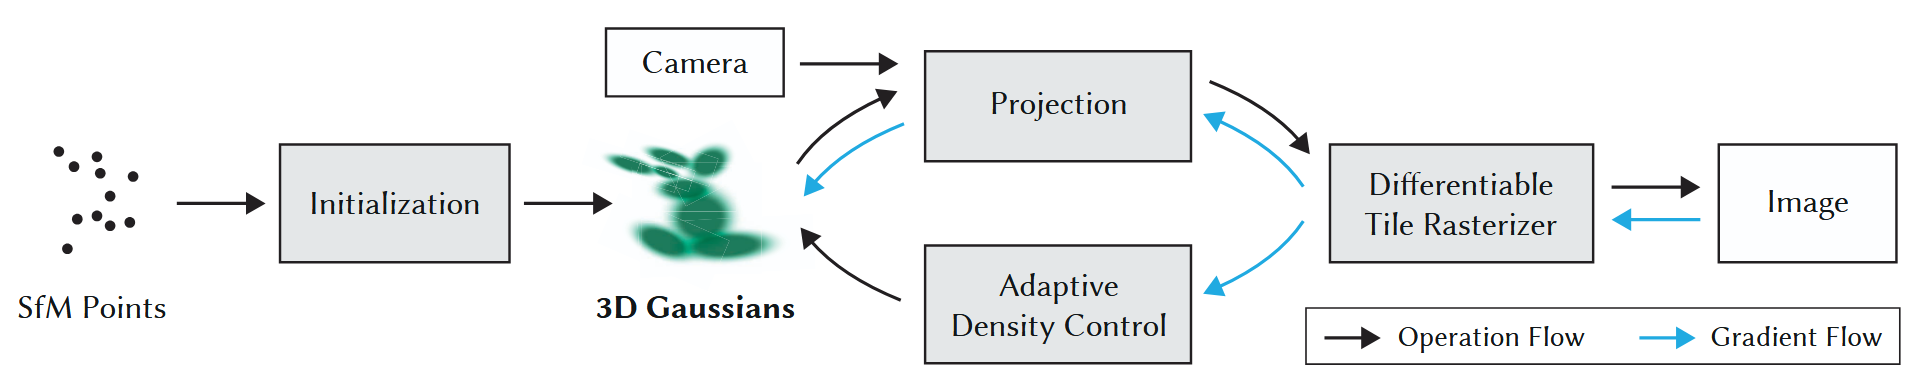
\includegraphics[width=0.92\textwidth]{figuras/kerbl2023_fig2.png}}
    \caption{Esquema do \textit{pipeline} do 3D Gaussian Splatting, incluindo inicialização a partir de pontos de SfM, projeção, rasterização diferenciável e controle adaptativo de densidade. Fonte: \cite{kerbl2023}.}
    \label{fig:3dgs_pipeline}
\end{figure}

A Figura \ref{fig:3dgs_comparison} reforça empiricamente esse reposicionamento do problema. A comparação evidencia que o método proposto pelos autores busca ocupar um ponto intermediário particularmente valioso para aplicações interativas: mantém uma qualidade visual elevada, ao mesmo tempo em que alcança taxas de renderização muito superiores às de abordagens implícitas de maior custo. Nesse sentido, a imagem não funciona apenas como ilustração de resultado, mas como síntese visual da principal tese do artigo: a representação explícita pode reformular de maneira favorável o equilíbrio entre fidelidade e desempenho.

\begin{figure}[H]
    \centering
    \fbox{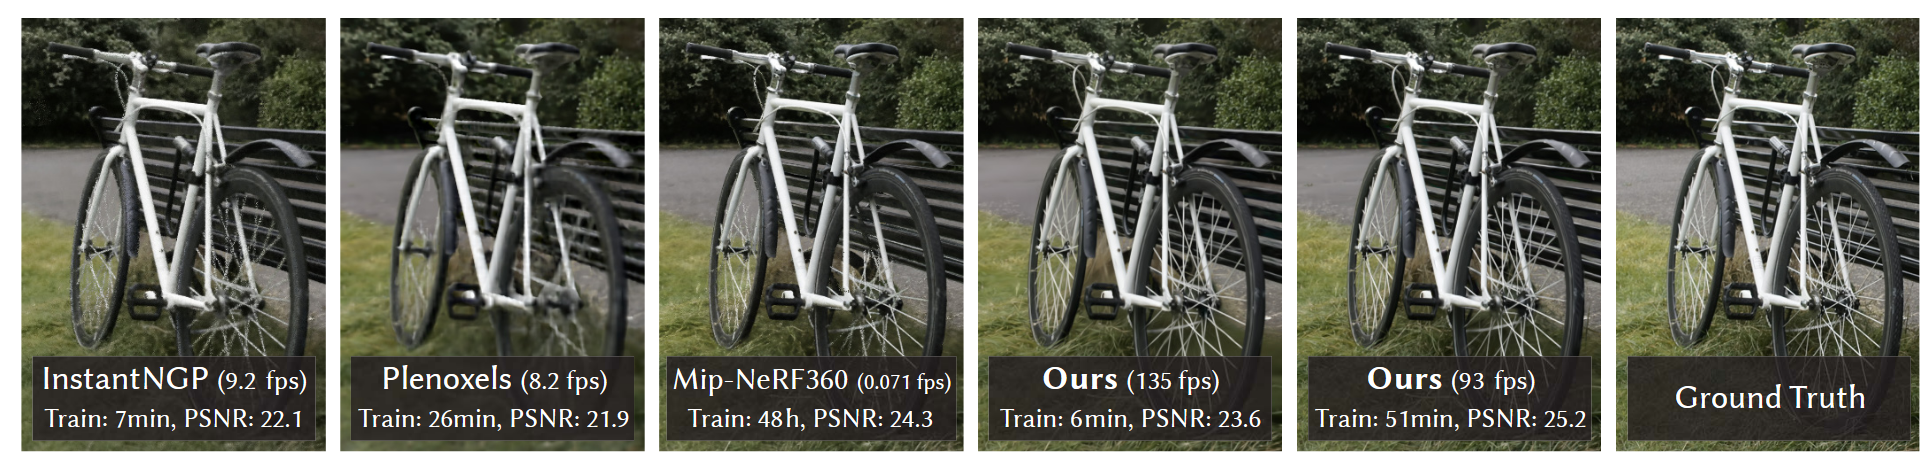
\includegraphics[width=0.97\textwidth]{figuras/kerbl2023_fig1.png}}
    \caption{Comparação visual e de desempenho entre métodos de síntese de novas vistas, evidenciando o compromisso entre tempo de treinamento, taxa de quadros e fidelidade visual. Fonte: \cite{kerbl2023}.}
    \label{fig:3dgs_comparison}
\end{figure}

No escopo desta pesquisa, o trabalho de Kerbl et al. é decisivo por tornar plausível uma estratégia de visualização mais aderente às restrições da realidade virtual. Embora o artigo não resolva, isoladamente, todos os desafios da implantação em ambientes imersivos, ele fornece a base metodológica mais forte para o uso de representações explícitas em cenários nos quais latência, taxa de quadros e previsibilidade de execução assumem um papel central.

\subsection{\textit{UE-GS: High-Quality 3D Gaussian Splatting Real-Time Rendering for Unreal Engine}}

Jin et al. \cite{jin2024} deslocam a discussão do nível estritamente algorítmico para o da integração prática em motor gráfico, ao abordar a renderização 3D Gaussian Splatting no Unreal Engine. Essa mudança de enfoque é altamente relevante para a presente pesquisa, pois o problema investigado não se encerra na capacidade de reconstruir ou sintetizar vistas de uma cena, mas se estende à implantação dessa representação em um ambiente real de desenvolvimento imersivo.

A Figura \ref{fig:uegs_qualitative} é pertinente porque evidencia o tipo de ganho que se torna especialmente relevante em motores gráficos: preservação de contornos, estruturas finas e detalhes locais que costumam se degradar quando a representação não está suficientemente bem integrada ao \textit{pipeline} de renderização. As ampliações em vermelho tornam a comparação mais objetiva, mostrando que a proposta dos autores se aproxima mais da referência do que a renderização 3D-GS tomada como base. Assim, a figura contribui para sustentar o argumento de que a discussão sobre representação de cena precisa ser acompanhada pela discussão sobre implantação em \textit{engine}.

\begin{figure}[H]
    \centering
    \fbox{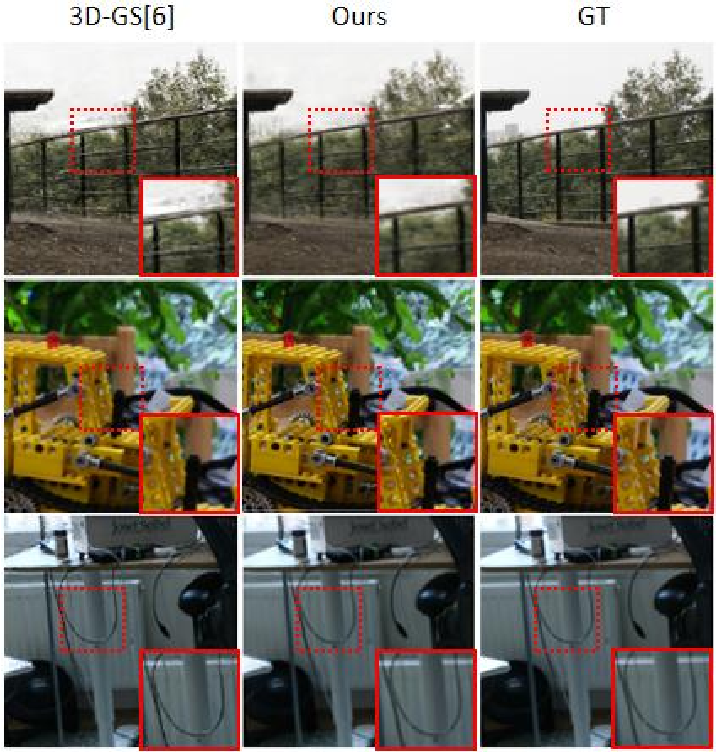
\includegraphics[width=0.50\textwidth]{figuras/jin2025_fig1.png}}
    \caption{Comparação qualitativa entre 3D-GS, a proposta de UE-GS e a imagem de referência, com ampliações destacando detalhes finos. Fonte: \cite{jin2024}.}
    \label{fig:uegs_qualitative}
\end{figure}

A principal pertinência do estudo decorre do fato de que motores gráficos como o Unreal Engine ocupam posição central na produção de experiências interativas, aplicações de visualização e ambientes virtuais. Assim, a integração do 3DGS à \textit{engine} constitui um passo importante na direção de \textit{pipelines} mais aplicáveis, em que a representação da cena não é apenas avaliada por métricas de qualidade de imagem, mas também por sua compatibilidade com ferramentas, rotinas de renderização e mecanismos de interação amplamente utilizados.

Ainda que o trabalho não se concentre especificamente na avaliação de conforto visual ou desempenho em dispositivos autônomos de VR, sua contribuição é metodologicamente significativa. Ele aproxima a literatura de representação neural da dimensão de implantação, aspecto particularmente importante para uma pesquisa cujo objetivo não é apenas compreender o estado da arte, mas examinar sua viabilidade prática em um fluxo de trabalho orientado à realidade virtual.

\subsection{\textit{VRSplat: Fast and Robust Gaussian Splatting for Virtual Reality}}

Tu et al. \cite{tu2025} apresentam um estudo tratando diretamente da adaptação de 3D Gaussian Splatting ao contexto da realidade virtual. Diferentemente de trabalhos que demonstram elevado desempenho apenas em visualização convencional, o VRSplat parte do reconhecimento de que a VR impõe exigências adicionais, como grande campo de visão, renderização estereoscópica, movimentos contínuos de cabeça e tolerância muito menor a artefatos temporais e inconsistências geométricas.

A Figura \ref{fig:vrsplat_pipeline} é particularmente relevante porque sintetiza a principal contribuição metodológica do VRSplat. Em vez de propor uma alteração pontual sobre o 3D Gaussian Splatting, o trabalho organiza um \textit{pipeline} integrado para realidade virtual, partindo de um modelo base eficiente, seguido de uma etapa de \textit{fine-tuning} com rasterização diferenciável livre de artefatos, até chegar a uma etapa de renderização com rasterização foveada. A figura evidencia, portanto, que a proposta dos autores não se limita à melhoria de qualidade visual isolada, mas busca conciliar robustez perceptual e desempenho compatível com aplicações imersivas.

\begin{figure}[H]
    \centering
    \fbox{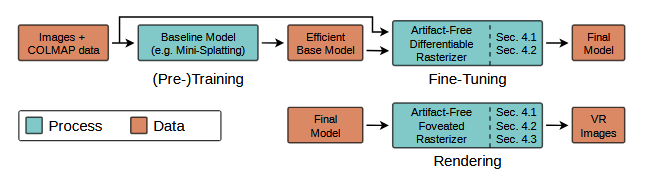
\includegraphics[width=0.80\textwidth]{figuras/tu2025_fig1.png}}
    \caption{Visão geral do pipeline do VRSplat para renderização de alta fidelidade
    em realidade virtual, incluindo modelo base eficiente, etapa de fine-tuning com
    rasterização livre de artefatos e renderização foveada. Fonte: \cite{tu2025}.}
    \label{fig:vrsplat_pipeline}
\end{figure}

Essa combinação evidencia uma mudança de maturidade da área: a discussão deixa de ser apenas “é possível renderizar rápido?” e passa a incorporar “é possível renderizar de forma estável e confortável em VR?”.

Para o presente trabalho, a principal contribuição do VRSplat está em mostrar que o uso de 3DGS em ambientes imersivos exige adaptações específicas, e não uma mera transposição direta de um método originalmente pensado para visualização monocular convencional. Essa observação é essencial, pois reforça a necessidade de que a avaliação experimental considere, além de PSNR, SSIM, LPIPS e FPS, aspectos qualitativos ligados à estabilidade visual e à robustez perceptual.

\section{Quadro comparativo dos estudos}

O Quadro \ref{qua:comparativo_estudos} sintetiza, de forma objetiva, as principais características dos estudos selecionados, com ênfase no tipo de representação adotada, no foco metodológico, na forma de avaliação dos resultados, nos dados ou cenários utilizados e nas limitações mais relevantes frente ao problema investigado. A análise detalhada de cada estudo é apresentada ao longo da seção, enquanto o quadro busca apenas explicitar, de maneira resumida, os principais pontos de convergência e distinção.

\begin{quadro}[H]
\centering
\footnotesize
\caption{Quadro comparativo dos estudos selecionados.}
\label{qua:comparativo_estudos}
\renewcommand{\arraystretch}{1.15}
\setlength{\tabcolsep}{3pt}
\begin{tabularx}{\textwidth}{|p{2.5cm}|p{2.5cm}|p{1.8cm}|p{2.3cm}|p{2.6cm}|X|}
\hline
\textbf{Estudo} & \textbf{Representação} & \textbf{Ênfase} & \textbf{Avaliação dos resultados} & \textbf{Dados/cenários utilizados} & \textbf{Limitação} \\
\hline

\textit{NeRF} \cite{mildenhall2020}
& Implícita
& Fidelidade
& PSNR, SSIM, visual
& Cenas sintéticas e reais
& Alto custo computacional \\
\hline

\textit{Instant-NGP} \cite{muller2022}
& Implícita
& Aceleração
& Qualidade e tempo
& Cenas variadas
& VR não tratada diretamente \\
\hline

\textit{VR-NeRF} \cite{xu2023}
& Implícita
& VR
& Fidelidade e FPS
& Ambientes capturados
& Dependência de multi-GPU \\
\hline

\textit{3D Gaussian Splatting} \cite{kerbl2023}
& Explícita
& Tempo real
& PSNR, SSIM, LPIPS, FPS
& Mip-NeRF360, Tanks and Temples, Deep Blending
& VR não abordada diretamente \\
\hline

\textit{UE-GS} \cite{jin2024}
& Explícita
& Engine
& Comparação visual e FPS
& Cenas integradas à engine
& VR autônoma ausente \\
\hline

\textit{VRSplat} \cite{tu2025}
& Explícita
& VR
& FPS, visual, estudo com usuários
& Cenas para VR
& Solução específica para 3DGS \\
\hline

\end{tabularx}
\end{quadro}

A análise sintetizada no Quadro \ref{qua:comparativo_estudos} evidencia, em primeiro lugar, uma transição metodológica importante no campo das representações neurais de cena. O trabalho de Mildenhall et al. \cite{mildenhall2020} estabelece a base conceitual das representações implícitas, demonstrando elevada capacidade de síntese de novas vistas, porém à custa de alto esforço computacional. Em seguida, Müller et al. \cite{muller2022} mostram que esse custo pode ser reduzido de forma significativa por meio de estratégias mais eficientes de codificação, tornando os campos neurais mais viáveis em contextos experimentais.

No recorte específico da realidade virtual, Xu et al. \cite{xu2023} representam um marco relevante ao demonstrarem que campos neurais podem ser empregados na captura, modelagem e visualização de espaços caminháveis com elevado grau de fidelidade. Entretanto, o estudo também evidencia que essa viabilidade depende de infraestrutura robusta, especialmente em termos de aquisição de dados e processamento multi-GPU. Em outras palavras, o VR-NeRF confirma o potencial científico da abordagem implícita em VR, mas também explicita os obstáculos práticos associados à sua adoção em cenários mais acessíveis.

Por outro lado, os estudos baseados em 3D Gaussian Splatting apontam uma mudança de ênfase em direção a representações explícitas mais compatíveis com
renderização eficiente. Kerbl et al. \cite{kerbl2023} reposicionam o debate ao mostrar que é possível obter elevada qualidade visual com taxas de renderização substancialmente mais adequadas ao tempo real. Jin et al. \cite{jin2024}, ao aproximarem essa representação do Unreal Engine, reforçam a importância da implantação em motores gráficos reais, enquanto Tu et al. \cite{tu2025} avançam na adaptação desse paradigma às exigências específicas da realidade virtual, como robustez perceptual, mitigação de artefatos e desempenho compatível com uso imersivo.

A inclusão das colunas referentes à avaliação dos resultados e aos dados ou cenários utilizados permite observar que os estudos não diferem apenas em sua formulação metodológica, mas também na forma como validam suas contribuições. Enquanto alguns trabalhos se apoiam predominantemente em métricas objetivas de qualidade e desempenho, outros incorporam comparações visuais, cenários capturados em ambiente real e até avaliações perceptuais com usuários. Essa distinção é particularmente relevante porque evidencia que, no contexto da realidade virtual, a análise de resultados não pode se restringir apenas à fidelidade de reconstrução, devendo também considerar estabilidade visual, robustez perceptual e viabilidade de execução.

Em conjunto, esses estudos mostram que a literatura evoluiu de modelos fortemente orientados à fidelidade visual para soluções cada vez mais comprometidas com viabilidade prática, integração e desempenho. Contudo, também revelam que ainda persiste uma lacuna entre a excelência técnica dos métodos propostos e sua adoção em um fluxo de trabalho aplicado, capaz de articular reconstrução neural, representação eficiente da cena e uso em realidade virtual sob restrições concretas de hardware e execução.

É nesse contexto que se insere o presente trabalho. Em vez de se restringir à análise isolada de uma única técnica, esta pesquisa propõe uma abordagem aplicada, voltada à avaliação da viabilidade de um \textit{pipeline} que envolva reconstrução neural, representação eficiente e integração em ambiente imersivo. Desse modo, busca-se compreender, de forma experimental, em que medida os avanços observados na literatura podem ser articulados de maneira coerente para atender simultaneamente aos requisitos de qualidade visual, desempenho e implantação prática em realidade virtual.

